%

% Cal Poly Thesis
% 
% based on UC Thesis format
%
% modified by Mark Barry 2/07.
%



\RequirePackage{ifpdf}
\documentclass[12pt]{ucthesis}



\newif\ifpdf
\ifx\pdfoutput\undefined
    \pdffalse % we are not running PDFLaTeX
\else
\pdfoutput=1 % we are running PDFLaTeX
\pdftrue \fi

\usepackage{url}
\ifpdf

    \usepackage[pdftex]{graphicx}
    % Update title and author below...
    \usepackage[pdftex,plainpages=false,breaklinks=true,colorlinks=true,urlcolor=blue,citecolor=blue,%
                                       linkcolor=blue,bookmarks=true,bookmarksopen=true,%
                                       bookmarksopenlevel=3,pdfstartview=FitV,
                                       pdfauthor={Jason Banich},
                                       pdftitle={Using Neural Networks to Assist in Prediction of Zebra Stripe Crosswalk Images},
                                       pdfkeywords={thesis, masters, cal poly}
                                       ]{hyperref}
    %Options with pdfstartview are FitV, FitB and FitH
    \pdfcompresslevel=1

\else
    \usepackage{graphicx}
\fi

\graphicspath{ {Images/} }

\usepackage[utf8]{inputenc}
\usepackage[T1]{fontenc}
\usepackage{lmodern} 

\usepackage{longtable}
\usepackage{amssymb}
\usepackage{amsmath}
\usepackage[letterpaper]{geometry}  %ORIG
%\usepackage[letterpaper,footskip=.25in]{geometry} %http://tex.stackexchange.com/questions/47202/how-to-keep-page-numbering-below-text
\usepackage[overload]{textcase}
\usepackage{multirow}
\usepackage{bigstrut}
\usepackage{tabularx}
\usepackage{adjustbox}
\usepackage{float}
\usepackage[section]{placeins} %maybe

\usepackage[disable]{todonotes} % notes not showed
%\usepackage[draft]{todonotes}   % notes showed

\bibliographystyle{abbrv}

\setlength{\parindent}{0.25in} \setlength{\parskip}{6pt}

\geometry{verbose,nohead,tmargin=1.25in,bmargin=1in,lmargin=1.5in,rmargin=1.3in}

\setcounter{tocdepth}{2}


% Different font in captions (single-spaced, bold) ------------
\newcommand{\captionfonts}{\small\bf\ssp}

\makeatletter  % Allow the use of @ in command names
\long\def\@makecaption#1#2{%
  \vskip\abovecaptionskip
  \sbox\@tempboxa{{\captionfonts #1: #2}}%
  \ifdim \wd\@tempboxa >\hsize
    {\captionfonts #1: #2\par}
  \else
    \hbox to\hsize{\hfil\box\@tempboxa\hfil}%
  \fi
  \vskip\belowcaptionskip}
\makeatother   % Cancel the effect of \makeatletter
% ---------------------------------------




\begin{document}

% Declarations for Front Matter

% Update fields below!
\title{Zebra Crosswalk Detection Assisted by Neural Networks}
\author{Jason Banich}
\degreemonth{June} \degreeyear{2016} \degree{Master of Science}
\defensemonth{June} \defenseyear{2016}
\numberofmembers{3} \chair{Dr. John Seng} \othermemberA{Dr. Franz Kurfess} \othermemberB{Dr. Philip Nico} \campus{San Luis Obispo}
\copyrightyears{seven}
\degree{Master Of Science} 
\field{Computer Science}


\todo[inline]{COMMENTS ARE ENABLED THIS IS NOT THE FINAL VERSION}
\todo[inline]{JASON - BE SURE THAT STRIPLETS HAS BEEN FIND AND REPLACED TO STRIPELETS FOR FINAL - CHECK CASE}
\todo[inline]{JASON - BE SURE THAT GRAY/GREY IS USED THE SAME EVERYWHERE  (GRAY IS CHOSEN ONE)}
\todo[inline]{JASON - Fix splitting of tables}
\todo[inline]{JASON - acknowledgements}
\todo[inline]{try to make images at the top of pages when I can}
\todo[inline]{JASON - Before paper is final, check all the charts and numbers are updated in results section}

\maketitle

\begin{frontmatter}

% Custom made for Cal Poly (by Mark Barry, modified by Andrew Tsui).
\copyrightpage

% Custom made for Cal Poly (by Andrew Tsui).
\committeemembershippage

\begin{abstract}
It can be difficult to guide yourself across a crosswalk when your visual capabilities are limited, which can be an everyday issue for someone with impaired vision. This paper aims to alleviate that issue for zebra stripe crosswalks by proposing an algorithm that incorporates multiple properties of zebra stripe crosswalks with a neural network to assist in quickly and accurately identifying a crosswalk in video and pictures taken from a smartphone camera.

This method improves the accuracy of zebra crosswalk detection in images. In a large dataset, it correctly identified 75\% of zebra crosswalks, while reducing the false discovery rate from 20\% without using neural networks to 2.26\% using this neural network method, and only incorrectly identifying 2.15\% of non-crosswalk images as crosswalks.
%\todo[inline]{JASON - add a bit more}
%\todo[inline]{JASON - two key numbers that are representative of what I found. this percent better or this percent more accurate}

\end{abstract}

\begin{acknowledgements}
I would like to thank my parents, Ann and Steve Banich, my girlfriend, Jenée Smith, and my thesis advisor, Dr. Seng, for their support.
%\todo[inline]{JASON - finish this, worded terribly}
\end{acknowledgements}


\tableofcontents


\listoftables

\listoffigures

\end{frontmatter}

\pagestyle{plain}

\renewcommand{\baselinestretch}{1.66}


\chapter{Introduction}
\label{intro}

Crossing the street can be dangerous for visually impaired individuals because orienting oneself is difficult without being able to use a visual marker. Visually impaired people must use non-visual cues such as listening for cars stopped at red lights and trying to walk in front of them. Vision processing could be applied to recognize the crosswalk to assist the user with limited vision. In order to increase the safety of blindly crossing the street, a phone app could allow the user to hold up their phone and get feedback about the location of the crosswalk. As they cross the street, they would receive feedback as to whether they were going off course. Developing a fast and reliable metric for detecting the crosswalk is the first step towards developing a vision processing phone app to aid the visually impaired.

There have been some investigations of zebra crosswalk detection, but none so far have used neural networks \cite{Coughlan2006}\cite{ZebraPhone}\cite{relatedworkbipolarity}. Neural networks are formed by a number of interconnected nodes that require training. Once trained, they are configured to a specific application to predict outcomes based on the inputs. Neural networks are being used for an increasing number of applications where patterns are difficult to decipher manually. Although the training process can be time consuming, neural networks run quickly once trained, which is a large benefit to any application where speed is a factor. 

Figure-ground segmentation has been used to separate the objects from the background scene. This technique can be applied to zebra crosswalks to allow the detection of potential stripelets in the image using geometric parameters \cite{Coughlan2006}. Adding neural networks to this discovery method allows us to use parameters to evaluate whether stripelets are part of a crosswalk, a task which would be difficult manually. This paper aims to use neural networks to improve the reliability of zebra crosswalk detection methods, by offering a different approach to the problem.

%-brief intro of NN-, explain basis of paper this is based on, explain training process, explain stripelets a bit, training parameters, one line about results, figure ground segmentation

%Introductory Paragraph - State the general field of interest in one or two paragraphs, and end with a sentence that states what study will accomplish. Do not keep the reader waiting to find out the precise subject of the dissertation.
%Explain your goals.
%overview of what will present}

\chapter{Background}
\section{Types of crosswalks}

There are many types of crosswalks (See figures \ref{fig:TypesOfXwalksFig} and \ref{fig:TypesOfXwalksRealFig} for some examples), the main two are zebra stripe crosswalks (sometimes called 'continental') and standard two line crosswalks. Two line crosswalks are more commonly used due to their simplicity, but zebra crosswalks are often used in more vulnerable intersections due to their benefits in visibility for drivers \cite{crosswalkTypeEvaluation}. Vision processing for the driving lane of a car has been done many times, and there is no substantial difference between that and a two line crosswalk. As such, algorithms that work for these are mostly interchangeable.

\begin{figure}[t]
\begin{center}
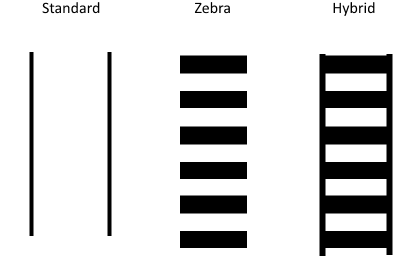
\includegraphics[width=10cm]{TypesOfXwalks.png}
\captionfonts
\caption[Three Types of Crosswalks]{A few types of crosswalks}
\label{fig:TypesOfXwalksFig}
\end{center}
\end{figure}

\begin{figure}[t]
\begin{center}
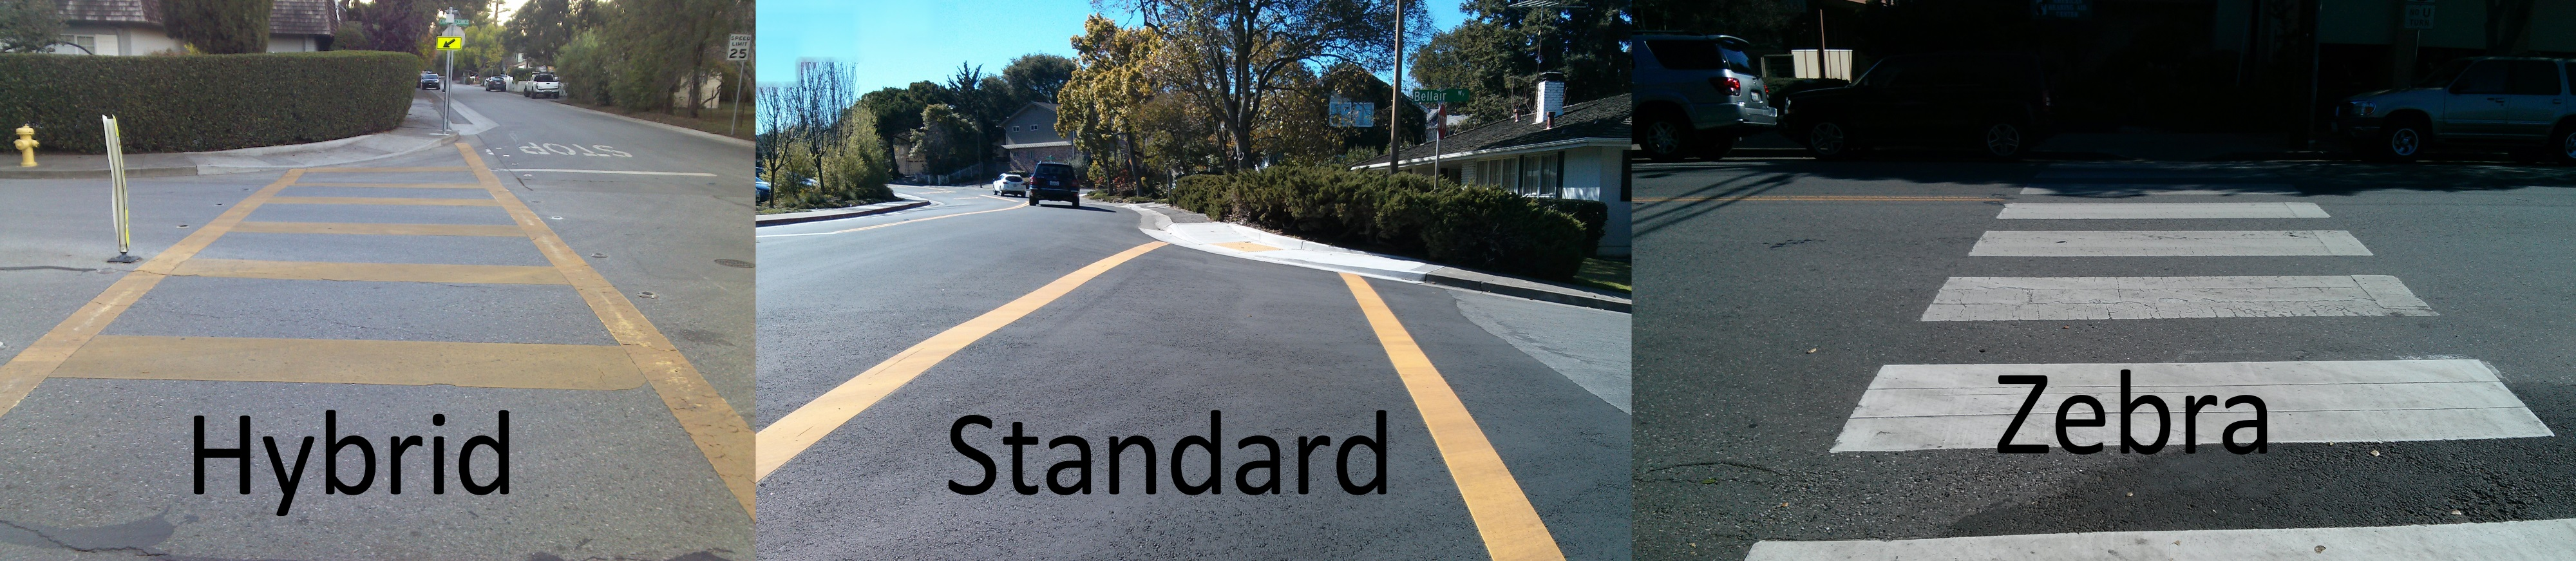
\includegraphics[width=13cm]{All3Types.png}
\captionfonts
\caption[Real Photos of Crosswalk Types]{Real world samples of the types of crosswalks}
\label{fig:TypesOfXwalksRealFig}
\end{center}
\end{figure}

\section{Neural Networks}
Neural networks are a type of machine learning that have been used recently for many vision applications such as image classification (See figure \ref{fig:DogWithHat}) and pattern recognition \cite{christianszegedy2014}, because they are useful for datasets with hard-to-detect patterns. Neural networks function using an interconnected network of neurons that work together to process the training data in order to discover a pattern or classification. Neural networks are well suited for many data sets that include lots of information that could be difficult to manually train a computer to categorize. One odd use case for neural networks is that they have been used to help determine which signals from a rat's brain should be used to trigger prosthetic limbs to move by measuring results of brain probes \cite{ratNeural}.

Neural networks are given a large amount of training data with known outputs. The network then runs over the dataset repeatedly, adjusting weighted parameters every iteration to reduce the amount of error in the predictions. Backpropogation of the data is also used in order to assist in training. Once the neural network is trained, the application can feed in new values and receive a prediction of the output.

\begin{figure}[t]
\begin{center}
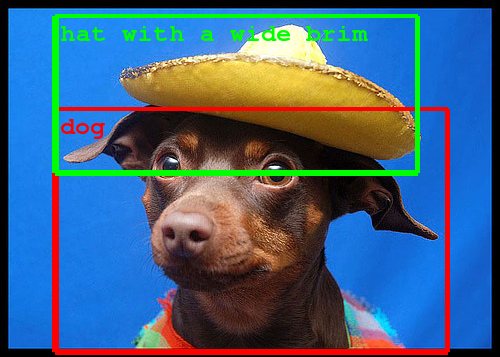
\includegraphics[width=10cm]{DogWithHat.PNG}
\captionfonts
\caption[Neural network classification example]{Neural network classification result\cite{christianszegedy2014}}
\label{fig:DogWithHat}
\end{center}
\end{figure}

\chapter{Related Works}
\label{Related Works}

\section{Standard Lane Following Algorithm}
As autonomous cars evolve into reality, there is a need for algorithms
to assist them in navigating and staying inside the lines. These
algorithms detect lines on the pavement, and
instructing the car to stay in the center. This is similar to
a two line crosswalk, the goal is to keep the user between the two
lines. However, with a crosswalk, the goal is to keep them inside the crosswalk, not necessarily centered.
One algorithm for lane following is as follows:
\begin{enumerate}
  \item Convert the image to grayscale
  \item Crop to the center portion of the image
  \item Identify the edges using an edge detection algorithm, and then draw the
  edges onto a new image
  \item Apply Hough line detection to find shapes in the edges
  \item Delete extraneous lines that were detected
  \item Apply and draw the discovered lines on the main image
\end{enumerate}
By following these steps, the image is processed and the lanes are returned,
which can then be used to direct the car to remain inside the lane \cite{SingleLane1}.


%https://www.researchgate.net/publication/4207389_Bipolarity_and_Projective_Invariant-Based_Zebra-Crossing_Detection_for_the_Visually_Impaired

\section{Crosswalk Detection Approach Using Pixel Bipolarity and Geometry}

Kyoto Institute of Technology's Uddin and Shioyama created a method of detecting zebra crosswalks using their geometric properties and the bipolarity of the images \cite{relatedworkbipolarity}. Their paper focuses on grouping large areas together that have high values of dark and/or light inside of them. Also, they use the projective invariant aka cross product to determine if the areas of light and dark in their image fit the pattern of a crosswalk. They then use the Fischer criterion to extract feature points in the image where the change from white to black (and vice versa) occur.

The steps are as follows:
\begin{enumerate}
   \item Convert to grayscale and split the image into 16x16 pixel groups.
   \item Find regions that are strongly bipolar by merging pixel groups that have a distance ratio within a threshold. The distance ratio is a measure of how similar the regions intensities are to each other in regards to bipolarity. A merged image is shown in figure \ref{fig:BipolarCrosswalk} section  (b).
   \item Once grouped, discard regions that don't exhibit enough bipolarity.
   \item Refine the segmentation by allowing larger groups to absorb smaller groups inside of them.
   \item Check where the region is in the image. If it is far to the left or right, classify it as such. If the bottom of the region is too high up in the image, discard it.
   \item Use a Fourier transform to check if the crosswalk angle is too extreme. If it is, throw it out. 
   \item Use Fischer criteria to find the feature points where the intensity changes drastically, determine that there are at least seven (which means there are four or more crosswalk stripes in the image), and then check the projective invariant criteria to see if it passes or is thrown out. 
   \item Repeat for each region until a match is found or all regions are exhausted.
\end{enumerate}
This method had decent results, with a high true positive rate (74 / 79), and zero false positives out of 34 other images. One downside of their method is that the image is required to have a minimum of four crosswalk stripes in the image to detect it, which means the majority of the crosswalk must be in the frame. Theoretically this method will work with a moderate amount of the crosswalk covered up (by other pedestrians or cars) as long as there are enough feature points in a vertical line in at least one area to detect the crosswalk. 

\begin{figure}[t]
\begin{center}
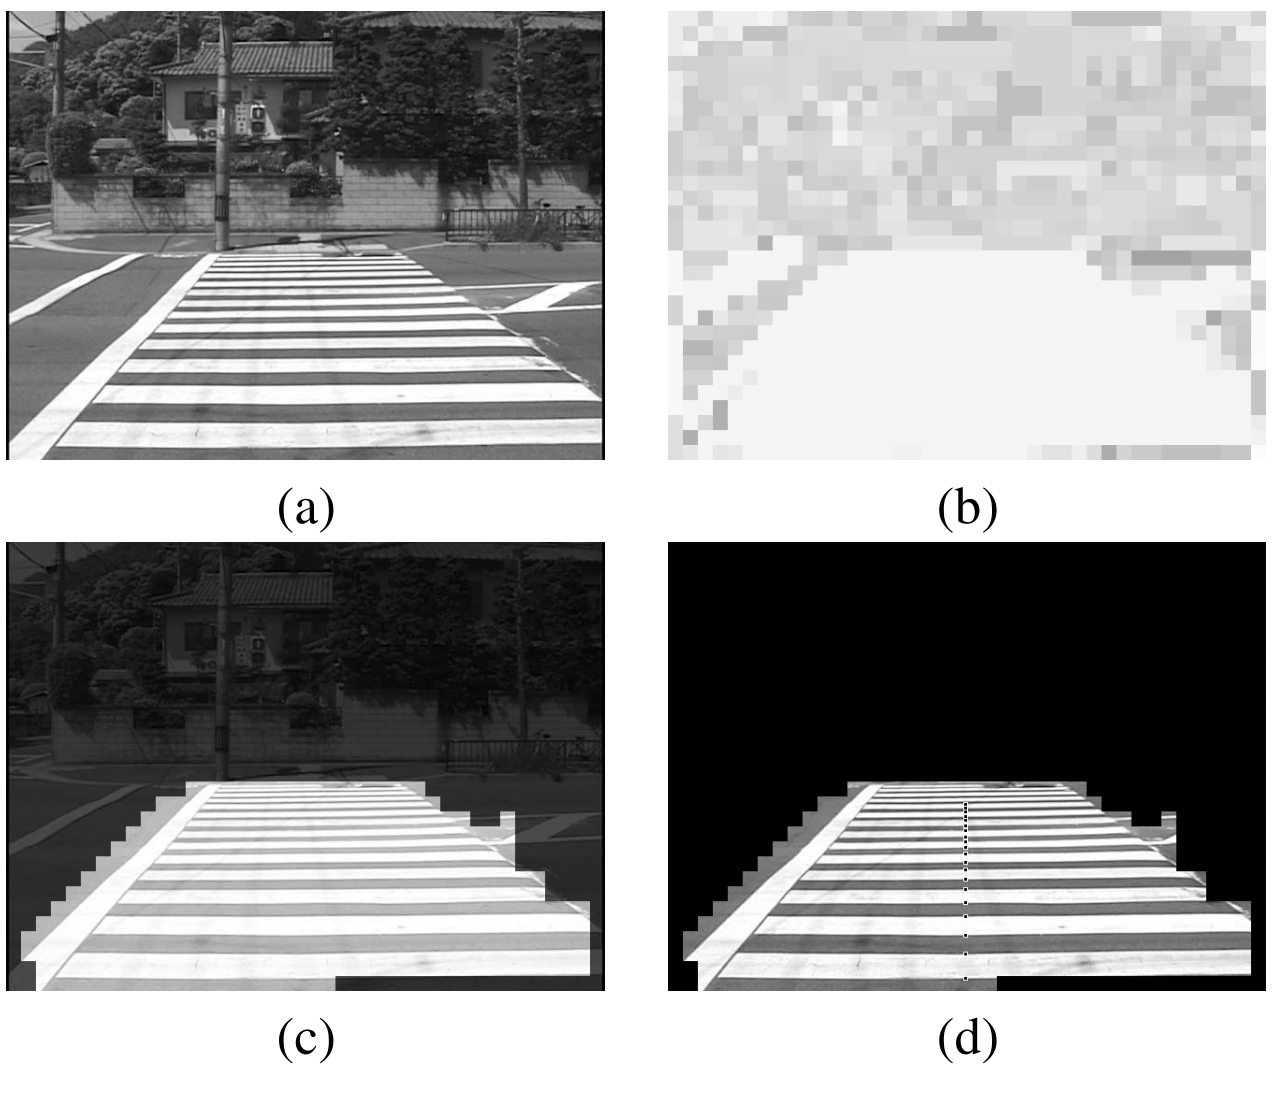
\includegraphics[width=10cm]{BipolarCrosswalk.png}
\captionfonts
\caption[Bipolarity and Projective Invariant detection example]{Steps of detecting a zebra crosswalk using Bipolarity and Projective Invariant: (a) gray scale image, (b) bipolarity of each segmented region, (c) original image highlighting the largest detected region, (d) extracted feature points shown on region}
\label{fig:BipolarCrosswalk}
\end{center}
\end{figure}




\chapter{Detecting Zebra Crosswalks}

\section{Properties of zebra crosswalks}

Zebra crosswalks have many properties that could be used to help identify them, one example would be the lengths of the crosswalk's edges. The edges are well defined in most images of crosswalks, so they can be collected rather easily, and have a distinct shape. Other qualities include the fact that painted stripes are typically homogeneous in the center in terms of pixel intensity. Zebra crosswalk stripes are also spaced a consistent distance apart. The horizontal lines in the crosswalk are all exactly parallel, and the side edges of each side of a zebra crosswalk should be parallel as well and point towards the vanishing point. Some of these properties will be recognized and used in later sections to uniquely identify zebra stripe crosswalks. 

\section{Coughlan Approach}
In Coughlan and Shen's 2006 paper \cite{Coughlan2006} about identifying zebra crosswalks, they propose a method for recognizing zebra stripe crosswalks using figure-ground segmentation.  Their method starts by converting the image to grayscale, shrinking it, and then blurring it slightly. Then, the derivative of image intensity is taken in the Y direction to find the pixels that look like top and bottom edges. The derivative assigns top lines a negative value, and bottom lines a positive value.  These edges are then greedily grouping together into larger line segments. The edges are then matched up with other edges that might fit together to be part of the same crosswalk stripe. They define a candidate stripe fragment feature as a 'stripelet.' A stripelet is defined as the combination of two line segments with the following properties: 
\begin{enumerate}
  \item The upper and lower segments have polarities consistent with a crosswalk stripe (upper is above lower).
  \item The two segments are roughly parallel.
  \item The segments have sufficient overlap in the X coordinate range.
  \item The vertical width of the stripelet must be between 2 and 70 pixels (determined value from their test images).
\end{enumerate}

\begin{figure}[t]
\begin{center}
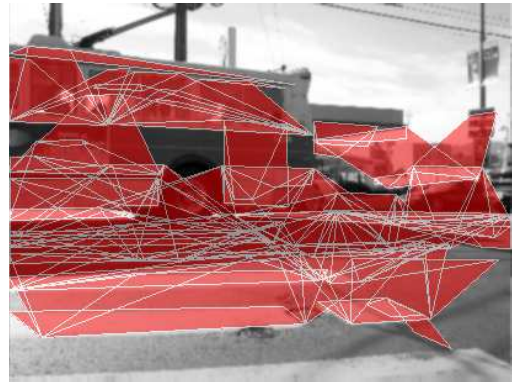
\includegraphics[width=10cm]{CoughlanStriplets.png}
\captionfonts
\caption[Coughlan Approach Stripelets]{Matched top and bottom pairs following the Coughlan Approach \cite{Coughlan2006}}
\label{fig:CoughlanStriplets}
\end{center}
\end{figure}

After matching up pairs of lines into stripelets, many stripelets are found, most of which are not part of the crosswalk (see figure \ref{fig:CoughlanStriplets}).

After extraction, unary and binary cues are used to determine if the stripelets are figure or ground. Their unary cue uses the fact that stripes lower in the image would be wider if they are part of a crosswalk. Coughlan and Shen found a relationship between the vertical width and vertical Y coordinate, as shown in the scatter plot in figure \ref{fig:CoughlanScatter}, a line drawn with a negative slope along a few points with low width and y value follows the lines that represent stripelets from the crosswalk. They then use a line fitting procedure to try and find an envelope line that fits that model. Once that line is found, they can use it to evaluate other stripelets. They look for longer stripelets that are close to the envelope in order to classify them as potentially a crosswalk stripelet. Additionally, a binary cue is used when the cross ratio test is applied to pairs of stripelets to check that all four lines are approximately parallel. Finally, the cross ratio is also used to verify that adjacent stripelets are within an acceptable distance from each other. 

\begin{figure}[t]
\begin{center}
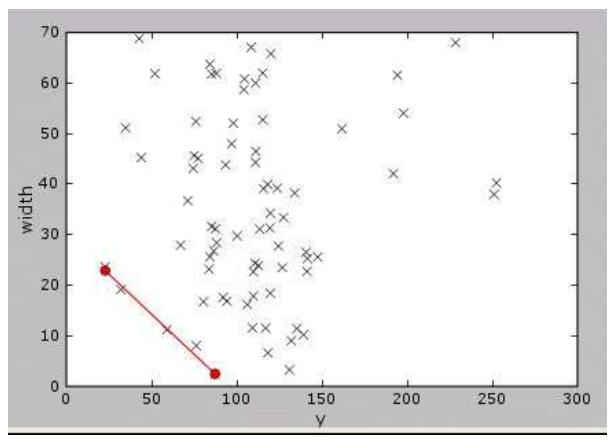
\includegraphics[width=10cm]{CoughlanScatter.png}
\captionfonts
\caption[Coughlan Scatterplot of Y and Vertical Width]{Scatter plot of vertical Y location and vertical width of stripelets \cite{Coughlan2006}}
\label{fig:CoughlanScatter}
\end{center}
\end{figure}

They ran this algorithm multiple times on each image with different envelope lines, and used the result that had the highest belief value of being correct. Their results are shown in figure \ref{fig:CoughlanResults}. These results were generated in few seconds per image. 

\begin{figure}[t]
\begin{center}
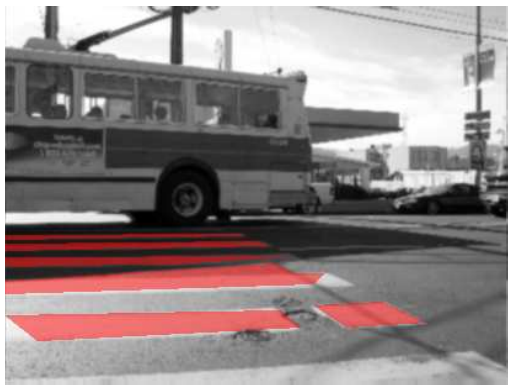
\includegraphics[width=10cm]{CoughlanResult.png}
\captionfonts
\caption[Coughlan Results]{Coughlan Results \cite{Coughlan2006}}
\label{fig:CoughlanResults}
\end{center}
\end{figure}

In their next paper in 2008 \cite{ZebraPhone}, they implemented this algorithm in Symbian C++ on a Nokia  N95 cell phone and obtained a true positive rate of 72\% and a false positive rate of 0.5\% on detected lines being predicted correctly as part of a crosswalk or not over a test set of 30 crosswalk images and 60 non-crosswalk images. Running on their 332 MHz ARM 11 processor running on 320x240 resolution pictures, they were able to obtain a processing speed of three frames per second with optimizations, compared to their processing speed on a PC with unoptimized code, and they believed the code could be further optimized as well. 

\chapter{Neural Network Background}
%JASON - More in depth than section in background, and more explanation of how they work}
%https://mattmazur.com/2015/03/17/a-step-by-step-backpropagation-example/  (simple example)
%http://home.agh.edu.pl/~vlsi/AI/backp_t_en/backprop.html //more complex example

%Neural networks are a type of machine learning that have been used recently for many vision applications such as image classification (See figure \ref{fig:DogWithHat}) and pattern recognition \cite{christianszegedy2014}, because they are useful for datasets with hard-to-detect patterns. Neural networks function using an interconnected network of neurons that work together to process the training data in order to discover a pattern or classification. Neural networks are well suited for many data sets that include lots of information that could be difficult to manually train a computer to categorize. One odd use case for neural networks is that they have been used to help determine which signals from a rat's brain should be used to trigger prosthetic limbs to move by measuring results of brain probes \cite{ratNeural}.

%Neural networks are given a large amount of training data with known outputs. The network then runs over the entire dataset repeatedly, adjusting weighted parameters of each of the inputs every iteration to reduce the amount of error in the predictions. Backpropogation of the data is also used in order to assist in training. Once the neural network is trained, the application can feed in new values and receive a prediction of the output

\section{History}
\label{History}
%http://www.andreykurenkov.com/writing/a-brief-history-of-neural-nets-and-deep-learning/
%http://www.springer.com/cda/content/document/cda_downloaddocument/9789401798150-c2.pdf?SGWID=0-0-45-1495021-p177264210
%yadav_2015

The origins of neural networks originate in 1943, when McCulloh and Pitts published "A logical calculus of the ideas immanent in nervous activity." They showed that simple neural networks could compute a wide array of functions with the same underlying method. A computer that worked as a neural network was created by Frank Rosenblatt and others, with a focus on pattern matching. In 1986, Rumelhard, Hinton and Williams published "Learning Internal Representation by Error Propagation," which popularized the backpropogation method of finding weights, and brought neural networks to the forefront \cite{BackpropHist}, \cite{yadav_2015}.


\section{Neural Network Basics - Feedforward}
\label{Neural Network Basics - Feedforward}
%example of a simple thing where why the parameters are weighted
The quintessential example of a neural network is a feedforward neural network. This network allows information to move forward only, from the inputs to the outputs. An example of a basic feedforward neural network is shown in figure \ref{fig:smallNN}. A series of weights are assigned to every connection, the inputs are fed through the network, multiplied by each respective weight, summed, and then fed to the next layer until the output values are generated. To train a feedforward network, one must either manually adjust the weights, or come up with a mathematical formula to do so. One such method is backpropogation \cite{feedforwardsource}. 

\begin{figure}[t]
\begin{center}
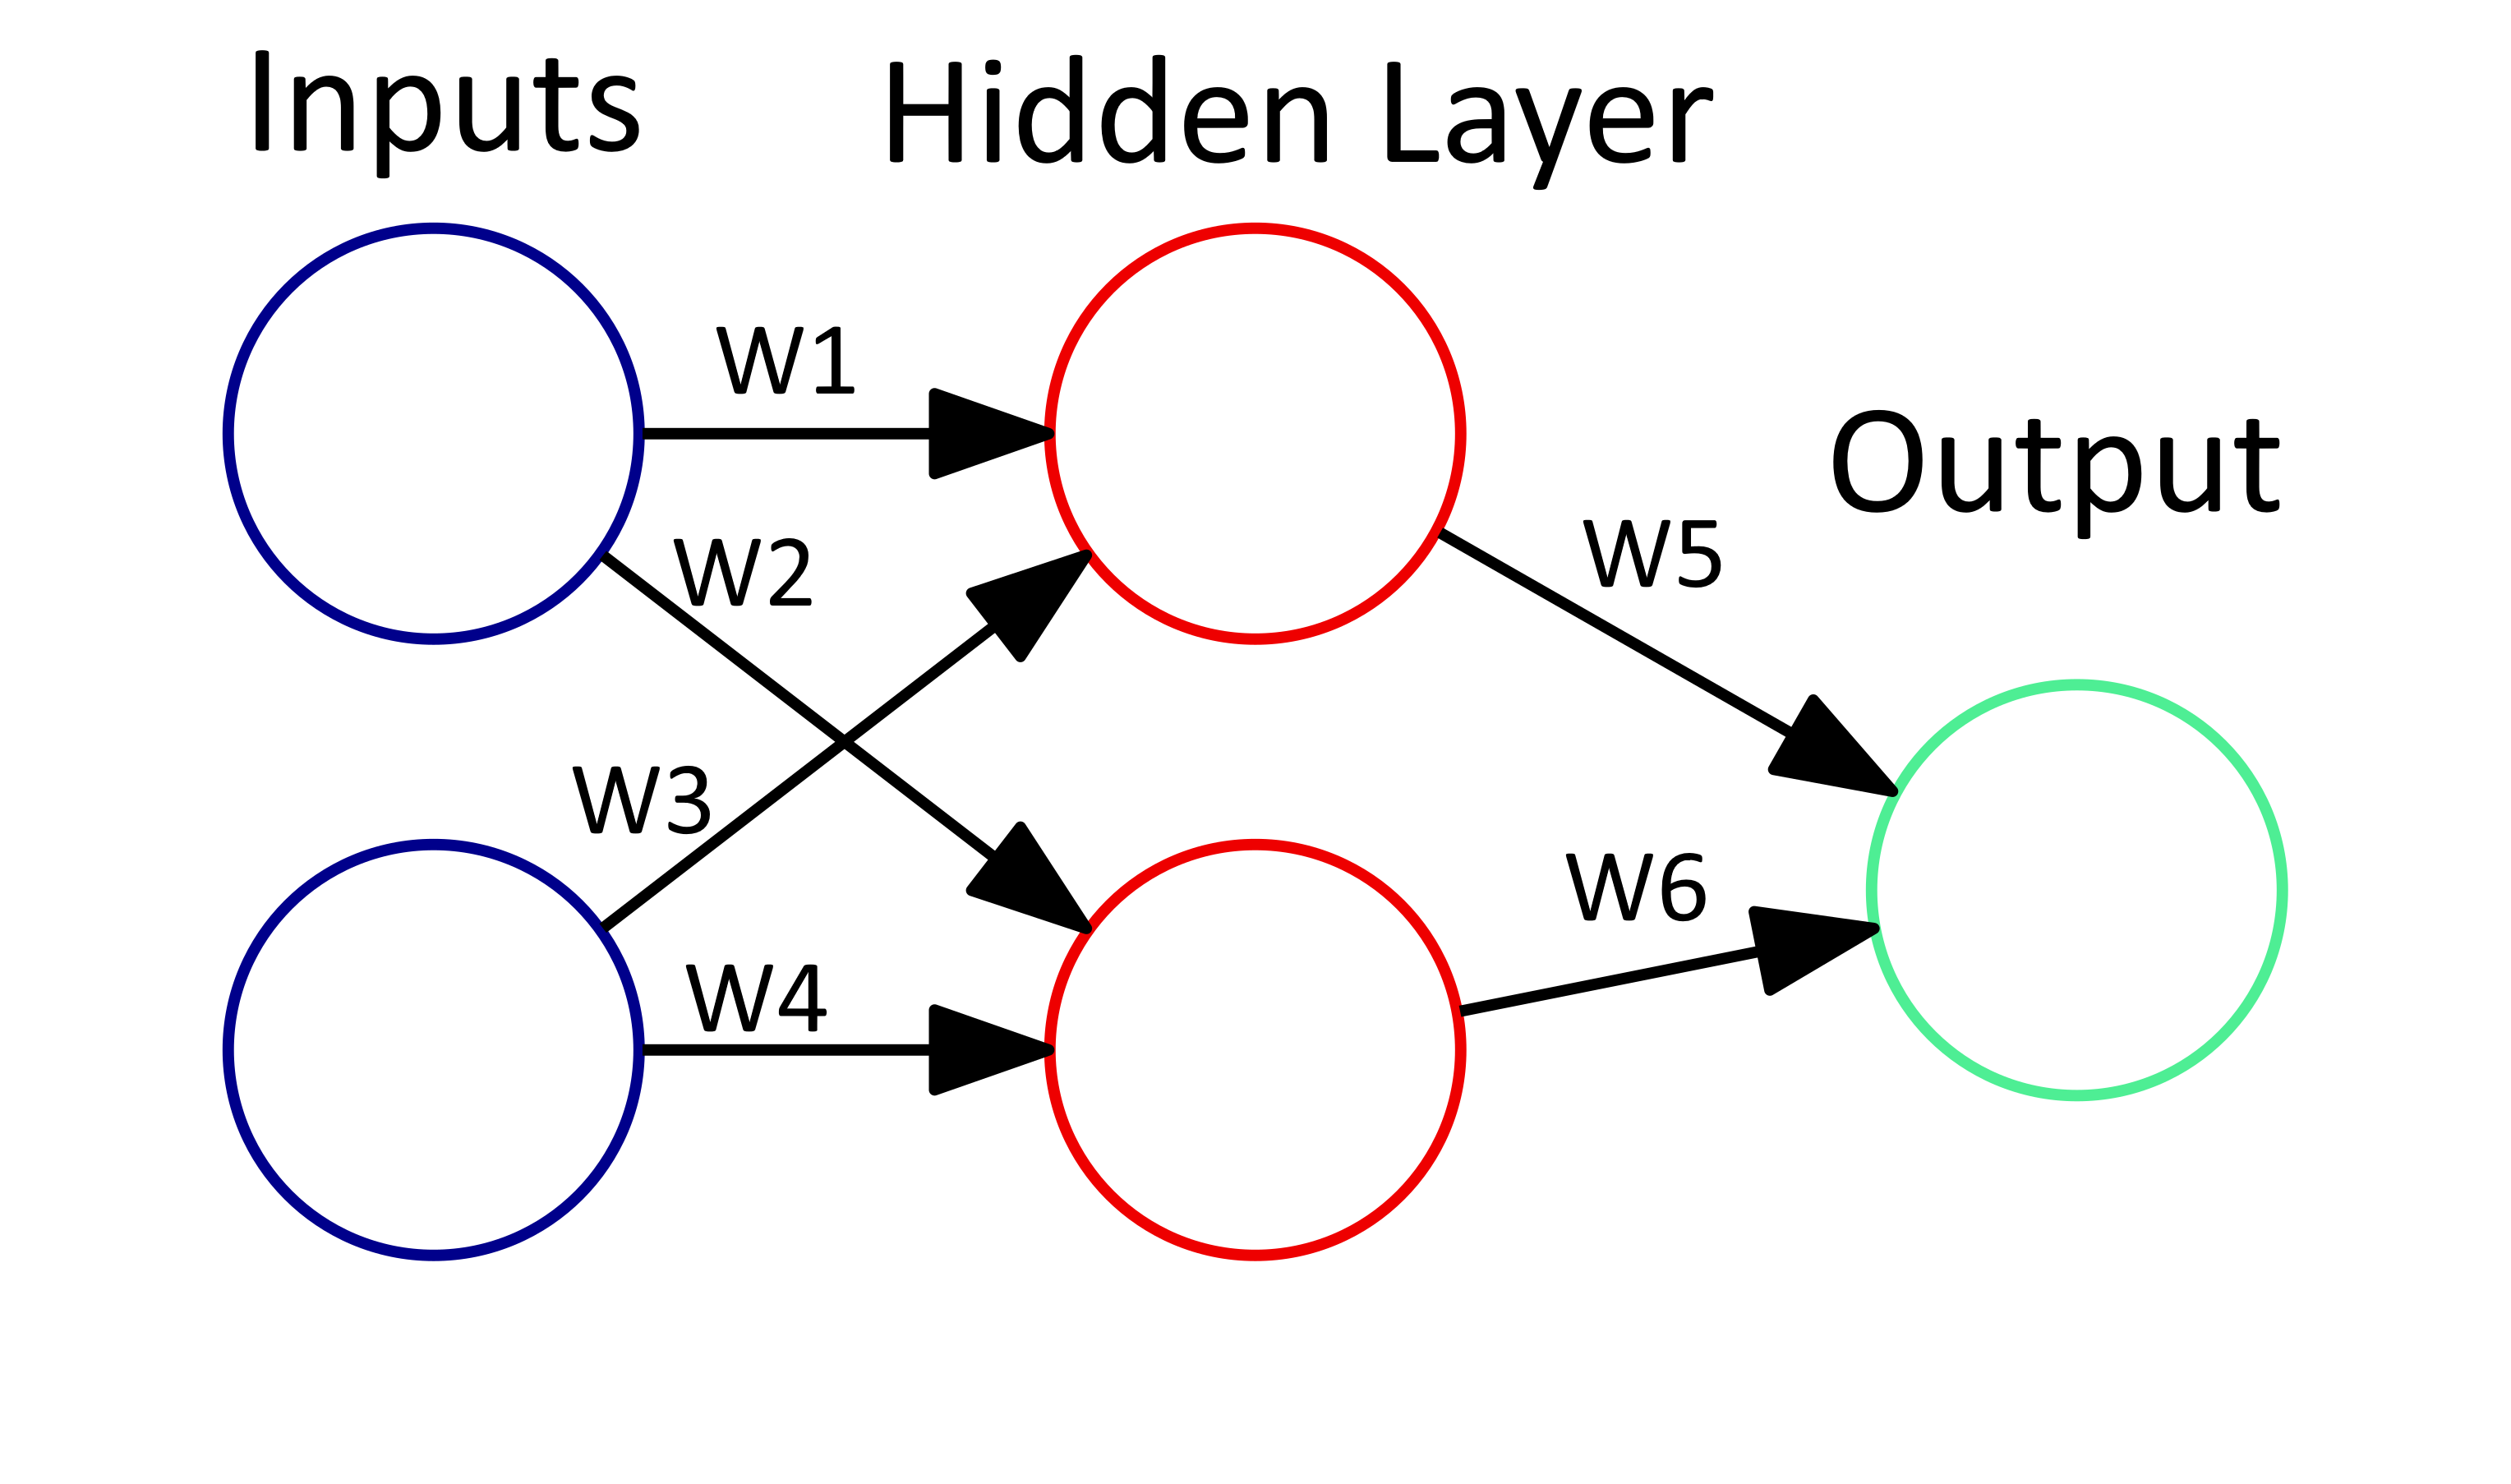
\includegraphics[width=10cm]{simpler.png}
\captionfonts
\caption[Small Neural Network Example]{Example of a small neural network with weights labeled}
\label{fig:smallNN}
\end{center}
\end{figure}

\section{Backpropagation Neural Network}
\label{Backpropagation Neural Network}
Backpropagation is a method of training neural networks by adjusting weights backwards through the network. It starts with weights for every link, and runs through them. The error on the output is calculated versus the expected output using the squared error function and the sum of the total error among all output nodes. Then, working from the outputs backwards, one works with all of the weights feeding into a prior node one at a time using partial derivatives and the chain rule. The reason the partial derivative is used is because the hidden layers all jointly affect the output nodes' error and must be taken into account. Once all of the weights are adjusted, the error should decrease and then the process is repeated until the error level is reduced to an acceptable level \cite{backpropositionPaper}. 

\chapter{Using Neural Networks to Detect Zebra Crosswalks}

\section{Input Image Constraints}
\label{Input Image Constraints}

Some image constraints were chosen for this scope of this paper because they would have been difficult to incorporate into this algorithm and were not necessary for a proof of concept implementation.

\begin{itemize}
\item All images are taken horizontally.
\end{itemize}

As detailed in future work, odd image angles can be very easily accounted for using the sensors of a phone, and the frame being horizontal makes image processing easier. Being able to assume that all true stripelets are horizontal removes them from the sample early on for being too vertical, or having a slope that is too far from the horizon. 

\begin{itemize}
\item All images contain crosswalks unaffected by shadows.
\end{itemize}

Shadows in a crosswalk create extremely strong lines that can interfere with the detection algorithm, as such they will be left for future work. 

\begin{itemize}
\item All crosswalks are white.
\end{itemize}

Yellow and white crosswalks have different pixel intensities, which may cause issues with the neural network training parameters, so in order to negate that issue, yellow crosswalks were excluded. 

\section{Algorithm Overview}
\label{Algorithm Overview}

\subsection{Stripelet Detection}

Following the method in the figure-ground paper \cite{Coughlan2006}, the frame is blurred slightly, and then converted to grayscale (Shown in figure \ref{fig:SlightlyBlurred}). 

\begin{figure}[t]
\begin{center}
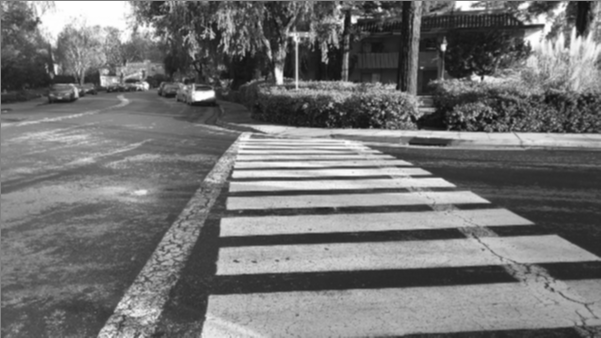
\includegraphics[width=7cm]{SlightlyBlurredInput.png}
\captionfonts
\caption[Grayscale Image]{Input image blurred and converted to grayscale}
\label{fig:SlightlyBlurred}
\end{center}
\end{figure}

The Sobel derivative is taken in the Y direction, leaving just the changes in the Y direction. The resulting pixels are either positive or negative, which signifies whether they are going from dark to light, or light to dark, giving us pixels that can be either the bottom or the top of the crosswalk. These are potential edges of crosswalks in the image (See figure \ref{fig:TopAndBottomSobel}). 

\begin{figure}[t]
\begin{center}
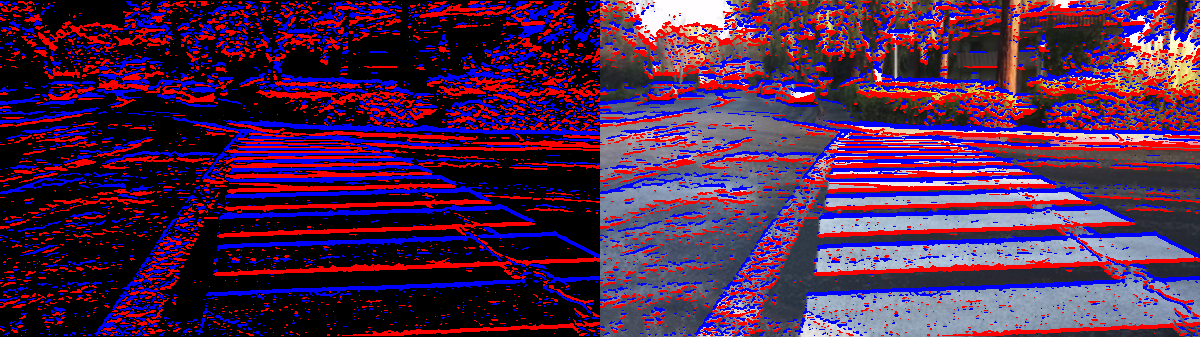
\includegraphics[width=14cm]{TopAndBottomSobel.png}
\captionfonts
\caption[Sobel Derivative of Crosswalk Image]{Sobel derivative of the image - positive values colored red, negative values colored blue}
\label{fig:TopAndBottomSobel}
\end{center}
\end{figure}

A standard method of Hough transform for line detection is then used to discover lines (figure \ref{fig:HoughLinesAfterMerge}). 

\begin{figure}[t]
\begin{center}
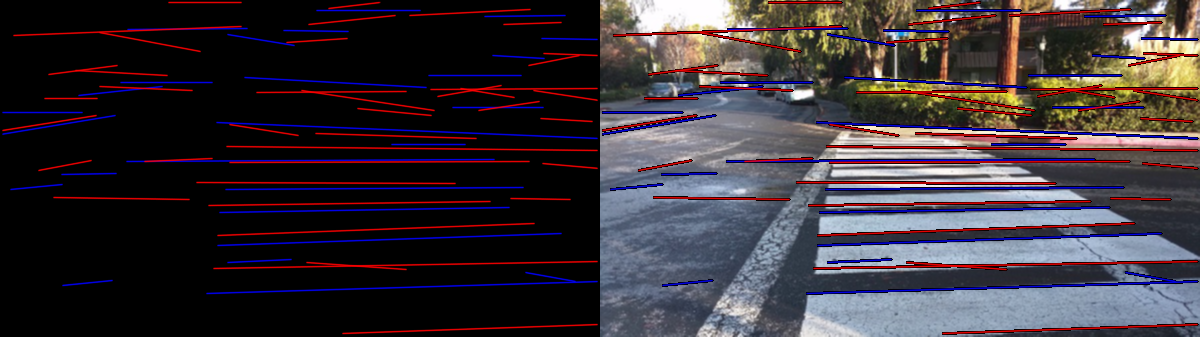
\includegraphics[width=14cm]{HoughLinesAfterMerge.png}
\captionfonts
\caption[Hough Line Transform Detection Result]{Lines detected using Hough transform on image from figure \ref{fig:TopAndBottomSobel} - blue is potential crosswalk top lines, red is potential crosswalk bottom lines}
\label{fig:HoughLinesAfterMerge}
\end{center}
\end{figure}

The generated lines are either defined as potential crosswalk top edges, or bottom edges. These potential edges are matched up against other edges (top vs bottom edges) to determine if they fit certain criteria to be considered stripelets. A stripelet is defined as an area bounded by a top and bottom line that follows certain constraints. The constraints used in Coughlan's figure-ground crosswalk paper \cite{Coughlan2006} are the same as used here: the top line is above the bottom line in the image, the two lines' slopes are very similar, the vertical width of the generated stripelet is between a defined cutoff value, and the two lines have sufficient X overlap. If all of these are true, then it is returned as a stripelet (See figure \ref{fig:UnculledStripelets}). 

\begin{figure}[t]
\begin{center}
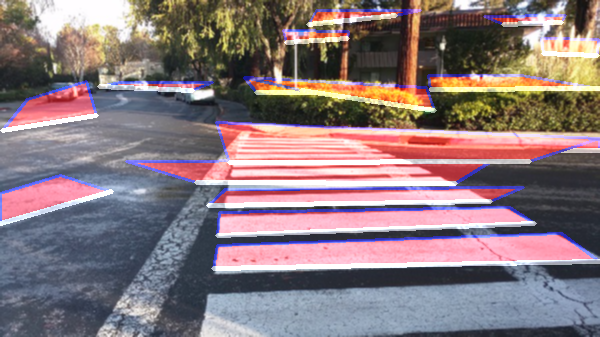
\includegraphics[width=7cm]{UnculledStripelets.png}
\captionfonts
\caption[All detected stripelets]{All of the stripelets detected after running the constraints on all the input lines from figure \ref{fig:HoughLinesAfterMerge}}
\label{fig:UnculledStripelets}
\end{center}
\end{figure}

\subsection{Neural Network Prediction of Crosswalk Stripelets}

%neural network based classification

At this point, the algorithm has generated a list of stripelets that are potentially part of a crosswalk. The inputs used for the neural network are a few parameters extracted from the image. The parameters are chosen because they possess characteristics that are believed may contribute towards helping identify a stripelet. A few sample parameters used are the stripelet's vertical/horizontal width, variance of the pixel intensity, and the lengths of the top and bottom lines. These numbers are calculated and then fed into the trained neural network, resulting in a very fast prediction as to whether or not that stripelet is part of a crosswalk.


Eleven different characteristics of the stripelets were chosen for use as the neural network parameters. The parameters are as follows:

\begin{enumerate}
   \item Bottom line length
   \begin{itemize}
     \item Description: The measure of the length of the bottom of the stripelet.
     \item Reasoning: Crosswalk stripelets are to have certain lengths, so this measure could help identify the validity of the stripelet.
   \end{itemize}
   \item Top line length
   \begin{itemize}
    \item Description: The measure of the length of the top of the stripelet.
    \item Reasoning: This value is similar to the bottom line length, and should pair well with the bottom length to give more information about the stripelet, as the two values are correlated.
   \end{itemize}
   \item Difference between top line length and bottom line length
   \begin{itemize}
     \item Description: The difference in length between the top and the bottom of the stripelet.
     \item Reasoning: Feeding in the difference between these measures explicitly could assist the neural network in using the difference. The bottom ought to be wider and the difference between the two should typically be a reasonably small number. 
   \end{itemize}
   \item Vertical stripelet width
   \begin{itemize}
     \item Description: The width of the stripelet vertically between the top and bottom lines.
     \item Reasoning: The vertical width of the stripelet is a useful factor because stripelets should have a certain vertical width that correlates with their top and bottom lengths, which would help define them as being part of a crosswalk.
   \end{itemize}
   \item Horizontal stripelet width
   \begin{itemize}
     \item Description: The width of the stripelet horizontally; the average length of the top and bottom lines.
     \item Reasoning: Similar to the vertical stripelet width, this parameter should correlate with the other parameters.
   \end{itemize}
   \item Vertical stripelet location
   \begin{itemize}
     \item Description: The vertical stripelet location (Y value of the stripelet center).
     \item Reasoning: The vertical stripelet location should help to correlate with other parameters to give a better prediction. For example, one might expect that a crosswalk stripelet higher in the image would be smaller, which would correlate this value with vertical and horizontal stripelet width. 
   \end{itemize}
   \item Variance of the stripelet pixel values
   \begin{itemize}
     \item Description: Pixel intensity variance within the stripelet.
     \item Reasoning: The pixel intensity variance should be lower for well painted stripelets, and high for stripelets that contain many different pixel values. This would be indicative of a non-crosswalk stripelet. 
   \end{itemize}
   \item Standard deviation of the stripelet pixel values
   \begin{itemize}
     \item Description: Square root of the variance.
     \item Reasoning: This measure may produce the same insights as the variance, and may allow a similar but simpler metric for the neural network to use.
   \end{itemize}
      \item Standard deviation of the pixel intensity of the area surrounding the stripelet
   \begin{itemize}
     \item Description: An area surrounding the stripelet is defined and the standard deviation of the pixel intensity in the area is found.
     \item Reasoning: The area around the stripelet should have a low standard deviation because it would be regular concrete without any lines for a crosswalk stripelet.
   \end{itemize}
      \item Standard deviation of the area surrounding the stripelet divided by standard deviation of the stripelet
   \begin{itemize}
     \item Description: The standard deviation of the area surrounding the stripelet divided by standard deviation of the stripelet.
     \item Reasoning: This ratio may help to give the neural network information about the relationship between the two measures.
   \end{itemize}
   \item Average stripelet pixel intensity divided by average pixel intensity of the area surrounding the stripelet
   \begin{itemize}
     \item Description: Average pixel intensity of the stripelet divided by the average pixel intensity of the area surrounding the stripelet.
     \item Reasoning: The stripelet pixel intensity should be much greater inside the stripelet than the area surrounding it, so this value could assist in finding which ratios are indicative of crosswalk stripelets or not. 
   \end{itemize}
\end{enumerate}

\subsection{Crosswalk Detection}

The stripelets that are predicted by the neural network to be part of a crosswalk are then checked one by one against the other stripelets through a manual feature comparison process. The compared features of the two stripelets are their average slopes, the horizontal pixel overlap, the vertical width of the stripelets, and the Y range overlap. The average slopes should be similar, the horizontal pixels should have a large amount of overlap, the vertical width of the stripelet which is lower in the image should be wider, as well as the horizontal width, and the Y ranges should have minimal overlap, if any. If two of the predicted crosswalk stripelets satisfy all of these constraints, then the image is declared to contain a zebra crosswalk. If all of the constraints fail to pass, then the image is not labeled a crosswalk. 

\subsection{Crosswalk Boundary Line Drawing}

In order to attempt to draw the boundary lines for the crosswalk, the edges from the stripelets that were positively identified as being part of a crosswalk are used. Three points are taken from the outer edges of the stripelets to assist in predicting the boundary as shown in figure \ref{fig:LinesAndEdgePoints}.  

\begin{figure}[t]
\begin{center}
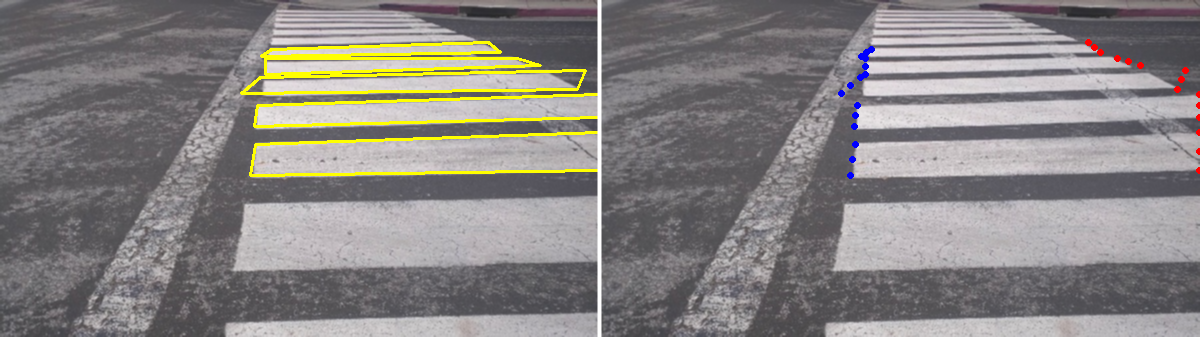
\includegraphics[width=14cm]{LinesAndEdgePoints.png}
\captionfonts
\caption[Crosswalk Detected Stripelets and points along their edges]{Left to right: (a) Stripelets used to detect crosswalk. (b) Points taken from the edges of the stripelets}
\label{fig:LinesAndEdgePoints}
\end{center}
\end{figure}

RANSAC line fitting is applied to these points in order to fit a line that is the approximation of the edge line, shown in figure \ref{fig:LinesUsingJustGoodStartAndEnds}. 

\begin{figure}[t]
\begin{center}
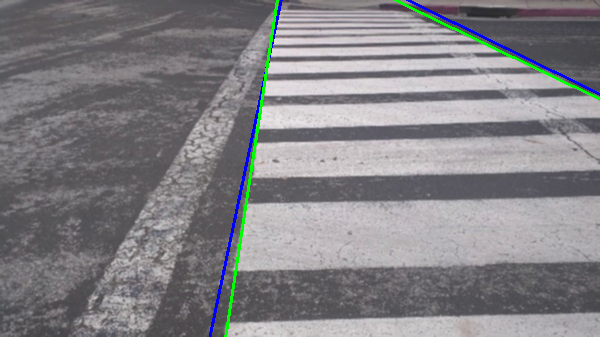
\includegraphics[width=7cm]{LinesUsingJustGoodStartAndEnds.png}
\captionfonts
\caption[Manually Entered and Estimated Line]{The green line is a manually drawn edge line, and the blue line is the estimated line}
\label{fig:LinesUsingJustGoodStartAndEnds}
\end{center}
\end{figure}


\chapter{Results}
\label{results}
%[inline]{tons of pictures. easy pictures, hard pictures, why they're hard}
%DONE{methodology section, like how neural networks were used, opencv section in methodology. cpu and clock speed and rate of processing}

\section{Methodology}

%Opencv/environment/language
\subsection{Environment}
This project was done entirely in OpenCV 3.0 using their C++ libraries. The computer used for this project was running Windows 8.1 on a Intel i5-2500K CPU with a maximum clock speed of 4.1 GHz. The OpenCV libraries are widely used and support a large amount of languages and platforms, including Apple iOS, Android, OpenCL, CUDA, as well as Mac, Linux and PC, which means that the code is easily ported to most any platform \cite{OpenCVPlatforms}. The input images were all read from saved video files on disk, and fed one by one into this project's algorithm. 

%what data was used, where it came from, what was trained, etc.
\subsection{Dataset}
%JeneePlz
The data used for the results were a selection of videos from multiple white crosswalks and streets without crosswalks taken at and around street intersections. The videos were taken at multiple times of day ranging from early morning to early night. For each crosswalk, five videos were taken going the same direction across the crosswalk. The videos were a high angle, a low angle, walking on the left side, on the right side, and a walking in the center.  Videos were given categories: time of day, angle of video, type of crosswalk, color, crosswalk title, and . Crosswalks were marked to be used only for training the neural network, and other crosswalks marked only to be used for evaluating results. The training set contained three hybrid crosswalks, six zebra crosswalks, and ten videos that did not include crosswalks. The result testing set contained three hybrid crosswalks, nine zebra crosswalks, and eighteen videos that did not include crosswalks. All data in the results section is generated from videos that were never used in the training process of the neural network. Over 14,000 stripelets were marked by hand as part of a crosswalk or not part of a crosswalk for use when training the neural network, and over 18,000 manually marked stripelets were used for the output. Each crosswalk video only used 20 frames, whereas videos without crosswalk may have used more. Hybrid crosswalks were included as well because they were working with the algorithm as well. 


%How Neural Networks are used here (explain some of the experimentation around different layers, and how they didn't do much)
\subsection{Neural Network Configuration}
%Jeneeplz
For this project, neural networks are used for the prediction of stripelets as either being part of a crosswalk or not. Neural networks require a set number of hidden layers with a set number of neurons, so some experimentation was done to determine these numbers. As shown in figure \ref{fig:Neural1png}, for this project, the final result was one hidden layer of 15 neurons. 

%D:\Users\SandyBridge\Dropbox\Thesis\My Paper Stuff\Results\Results of NN Training with diff neurons.xlsx
%    \begin{table}[t]
%%        \begin{longtable}{| r | r | r | r |}
 %       \hline
 %       Neurons in Hidden Layer & True Positive Rate & False Positive Rate & q-value \bigstrut\\
 %       \hline
 %       15 & 74.42\% & 2.36\% & 0.086 \bigstrut\\
 %       \hline
 %       \caption[Selected Neural Network Configuration Results]{Stripelet identification results from neural network training with selected hidden layer configuration}
 %       \label{tab:NN-HiddenLayersResults} 
 %       \end{longtable}
 %   \end{table}

There is no real consensus on exactly how many hidden layers and neurons should be used in the perfect neural network configuration. The different rules of thumb\cite{Heaton:2008:INN:1502373} have been that no more than one hidden layer is typically needed, and the number of neurons should be between the number of inputs and the number of outputs, and layers must have more than one neuron. With those being the guidelines, one hidden layer with a number of neurons mostly ranging from the number of inputs to the number of outputs was chosen with a range from 2 to 22 neurons in the hidden layer. Subsets of these training parameters were tried as well, with none having better results than using all eleven parameters. 



As shown in appendix table \ref{tab:NN-HiddenLayersResultsAPP}, some configurations were better than others, but none by much. The configuration with 15 hidden layers had the lowest false positive rate of 2.36\%, so it was chosen as the configuration to be used for the rest of this project. This fits with the original assumption that the number of neurons should be between the number of inputs and outputs as shown in figure \ref{fig:Neural1png}. 

\begin{figure}[t]
\begin{center}
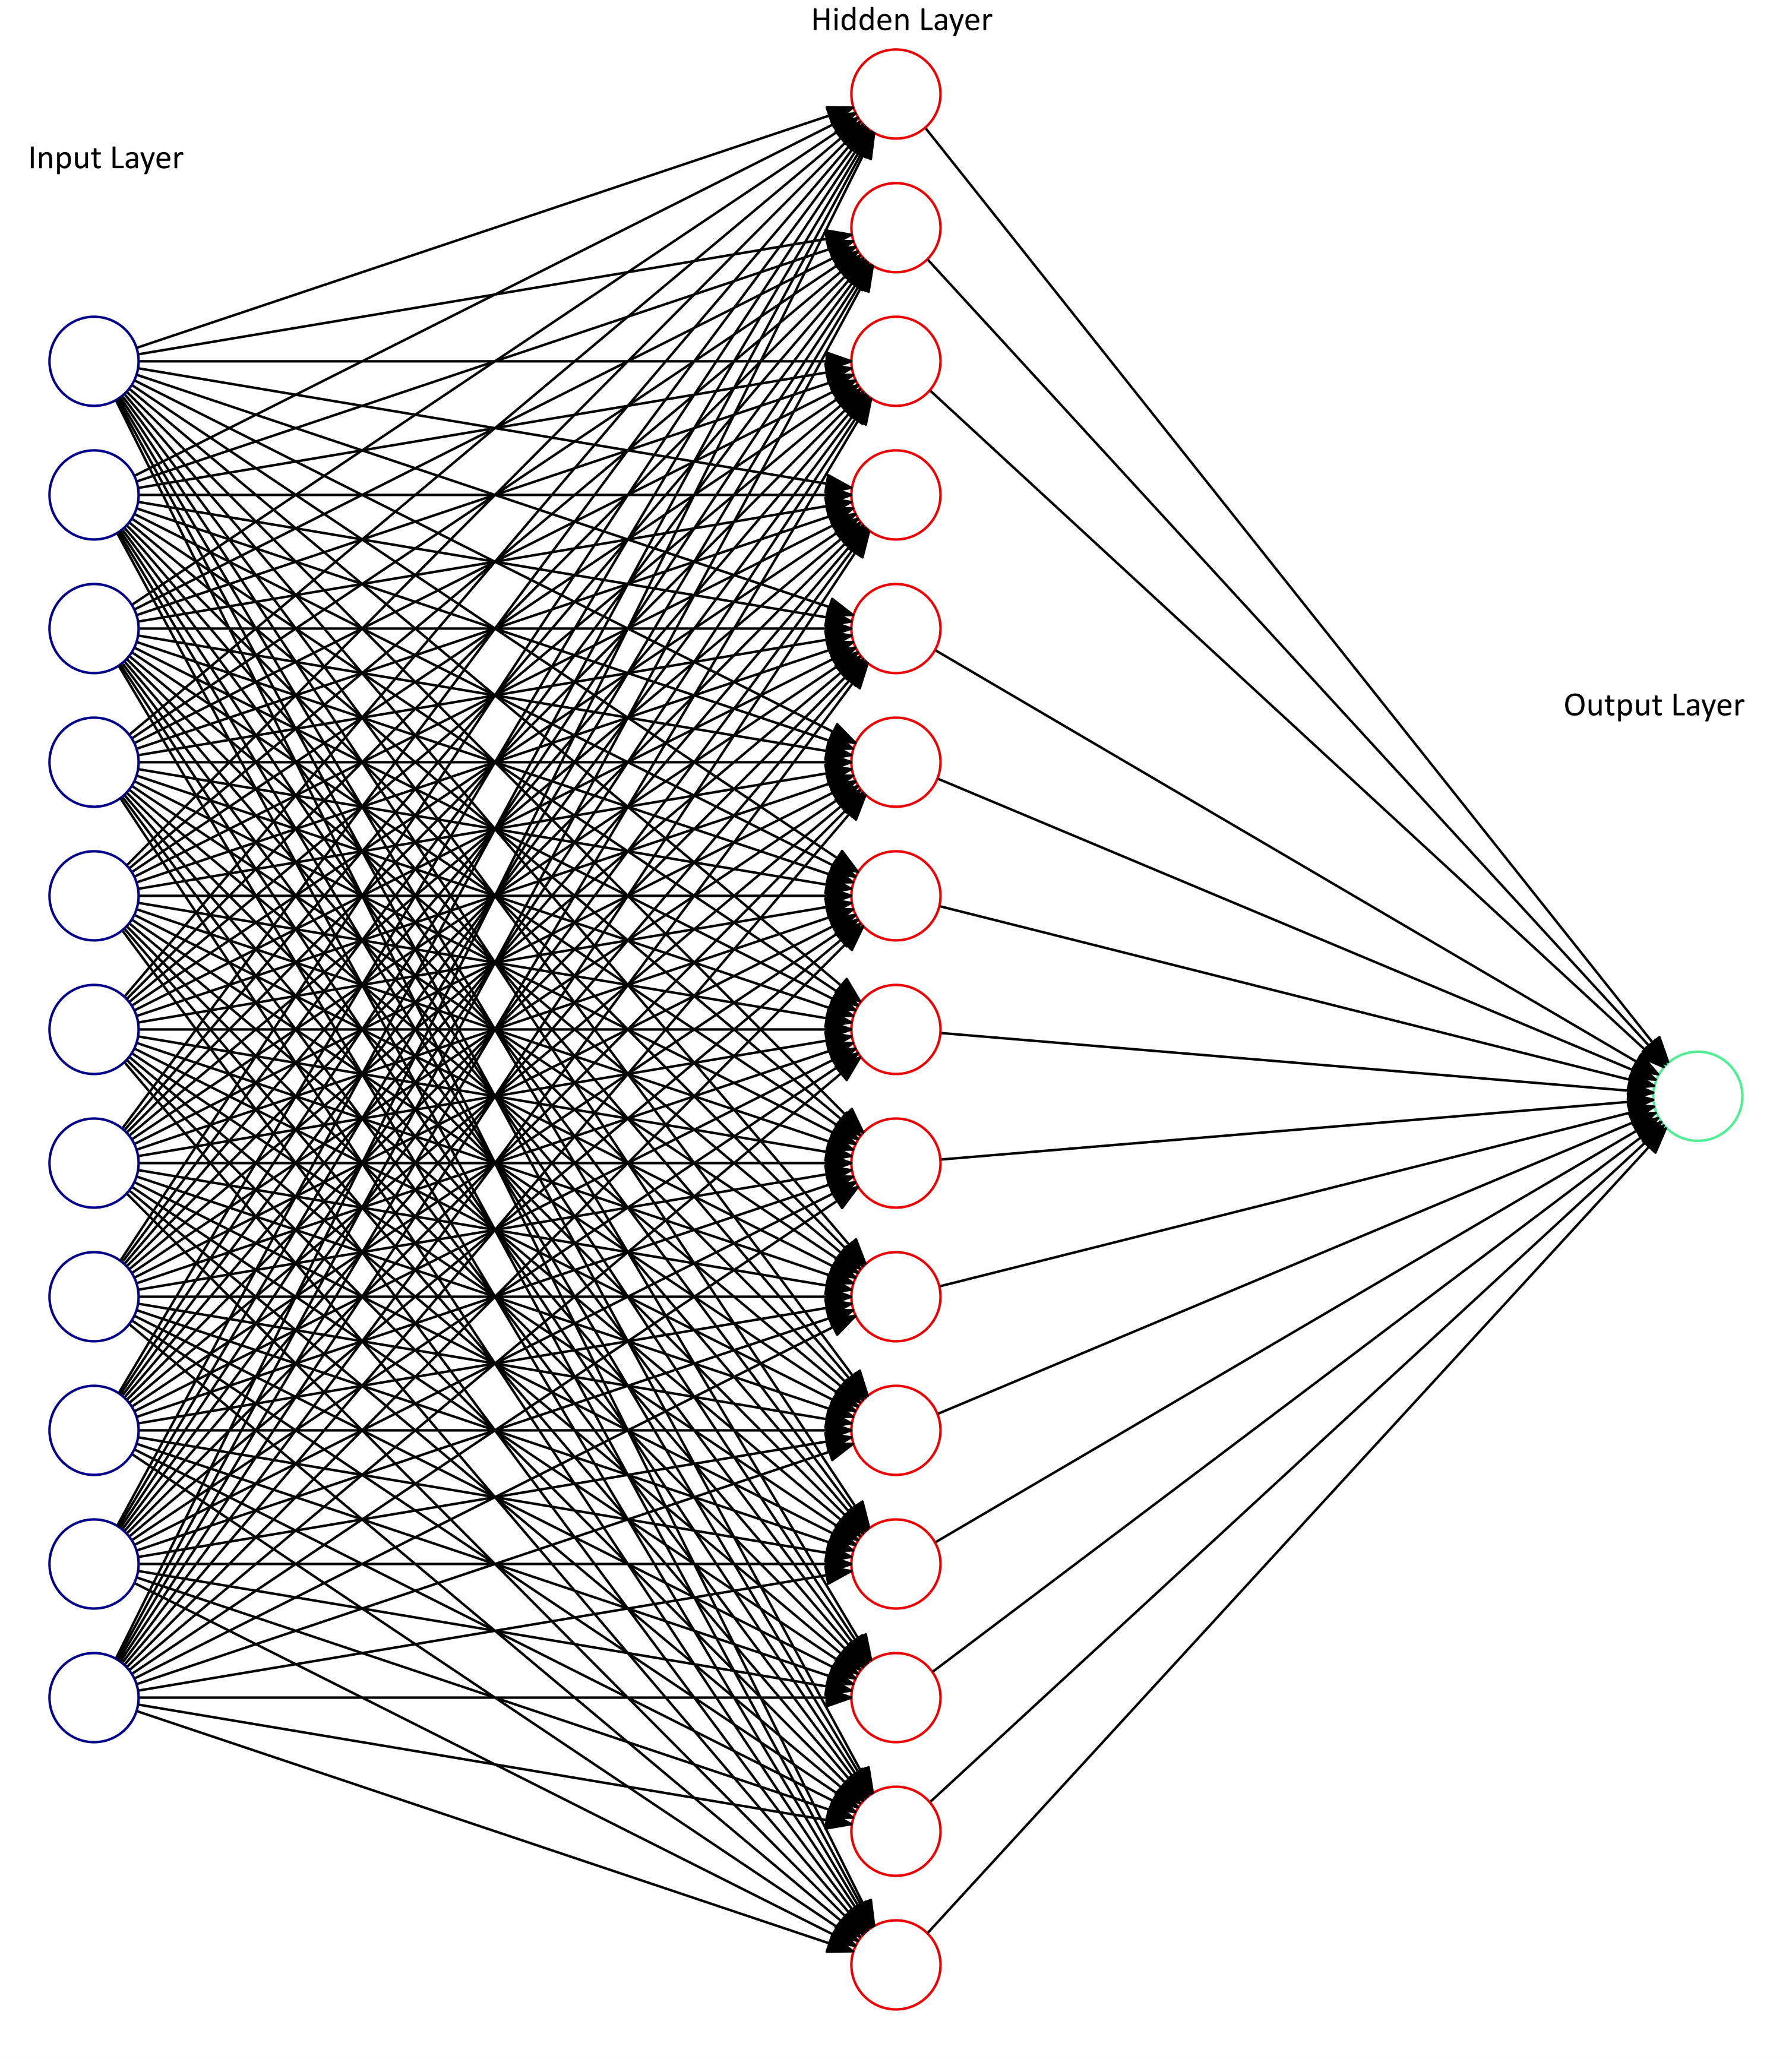
\includegraphics[width=10cm]{ChosenNN2.png}
\captionfonts
\caption[Final Neural Network Configuration]{Final neural network configuration showing input layers, hidden layers, and output layers}
\label{fig:Neural1png}
\end{center}
\end{figure}

\clearpage

\subsection{Neural Network Results}
%JeneePlz
%This is the results for different videos and their neural network results

    \begin{table}[t]
        \begin{longtable}{|r|r|r|r|}
        \hline
        Number of Stripelets & True Pos Rate & False Pos Rate & Q-Val \bigstrut\\
        \hline
        19461 & 77.61\% & 3.57\% & 0.1663 \bigstrut\\
        \hline
    
        \caption{Neural Network results over stripelets in final dataset}
        \label{tab:nnresultsoverall} 
        \end{longtable}
    \end{table}


The neural network training of the crosswalk stripelets used many different input parameters to predict the output. The metric used for evaluating the parameters was finding the true positive and false negative rates, as well as the false discovery rate (also known as q-value). The true positive rate is calculated by dividing the number of crosswalk stripelets that were predicted correctly as stripelets over the total number of crosswalk stripelets. The false positive rate is calculated by dividing the number of non-crosswalk stripelets predicted as stripelets out of the total number of non-crosswalk stripelets. The q-value is found by dividing the number of false positives by the number of stripelets that were predicted to be part of a crosswalk. Table \ref{tab:nnresultsoverall} shows the neural network prediction rates over the entire result set. Only 16\% of the positive results were incorrect. 
    




\subsection{Crosswalk Detection}
Once the neural network has finished culling stripelets, the remaining stripelets are then fed through the crosswalk detection algorithm. The results are again categorized by type of crosswalk, time of day, etc. 

\subsubsection{Effect of Different Video Angles}

There were five different angles used for the videos of the crosswalks, with 340 frames of video at each angle across many crosswalks. Examples of each angle are shown in figure \ref{fig:AllFiveAngles}. The low angle had worse correct prediction rates than the others, as shown in table \ref{tab:downbad}. The reason for this is that the cell phone camera was angled too low to capture enough stripelets for a positive identification. A few examples are given in figure \ref{fig:downBadPic}. The poor results from the bad video angle show that in an actual use case, that angle must be disallowed. The user could be trained to hold the cell phone camera at the proper angle, and if they did not, the sensors would allow the application to notify the user to adjust the camera angle. Because of this, the videos taken at that downward angle will be removed from the overall dataset. 

\begin{figure}[t]
\begin{center}
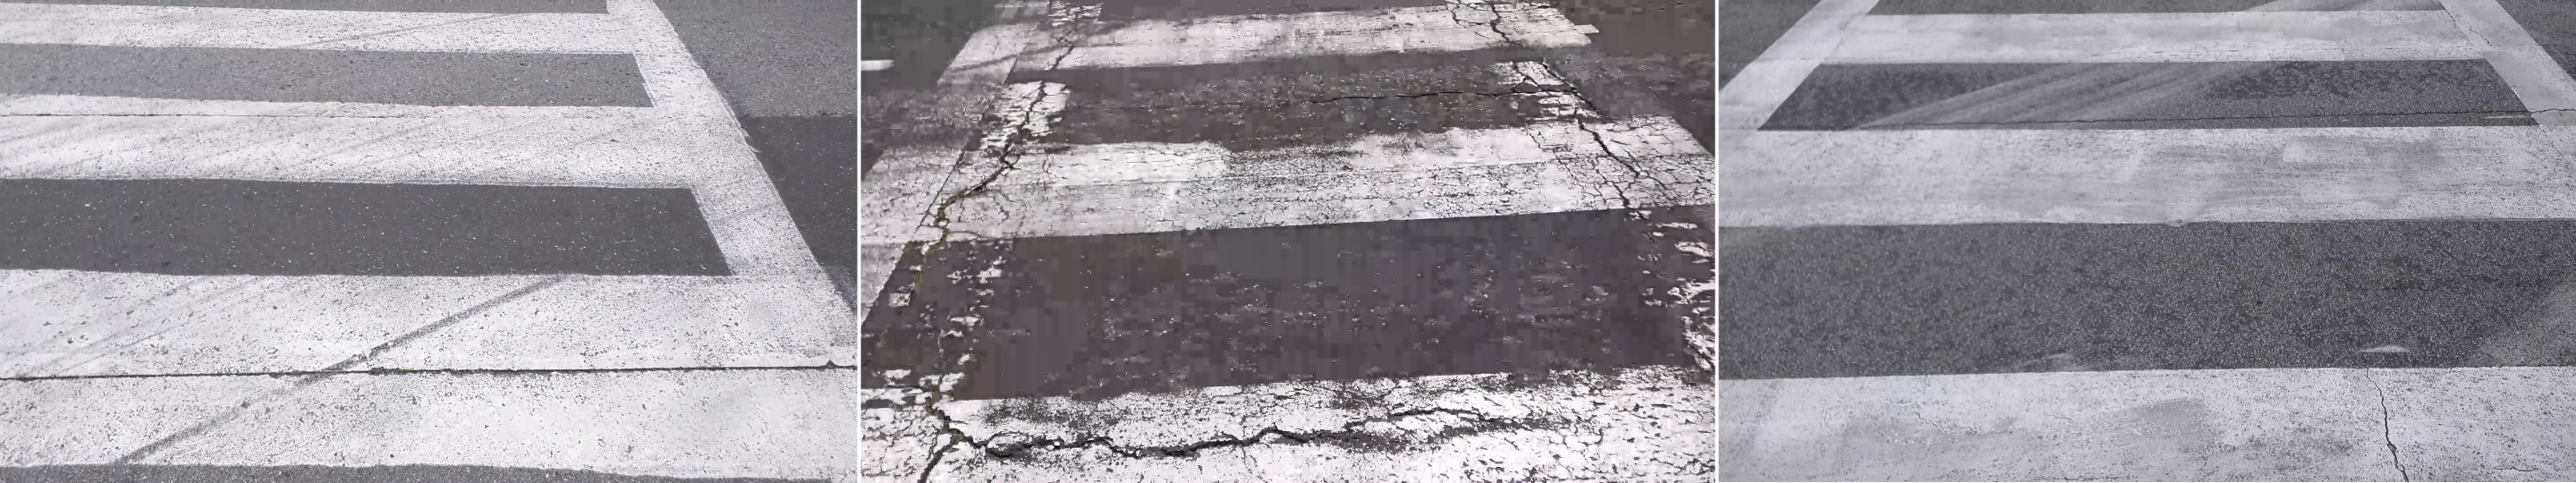
\includegraphics[width=15cm]{DownBad.png}
\captionfonts
\caption[Low Angle Video Examples]{Examples of the low angle video that garnered poor results}
\label{fig:downBadPic}
\end{center}
\end{figure}

\begin{figure}[t]
\begin{center}
\includegraphics[width=15cm]{AllFiveAngles.png}
\captionfonts
\caption[All Five Different Crosswalk Angles]{All five angles which videos were taken of the crosswalks. Left to right: (a) Low Angle (b) Left Side (c) Standard (d) Right Side (e) High Angle}
\label{fig:AllFiveAngles}
\end{center}
\end{figure}

\begin{table}[t]
    \begin{longtable}{|r|r|r|}
    \hline
    Camera Angle & True Positive Rate & False Positive Rate \bigstrut\\
    \hline
    Low Angle & 45.33\% & 0.00\% \bigstrut\\
    \hline
    Left Side & 75.33\% & 1.33\% \bigstrut\\
    \hline
    Standard & 77.67\% & 0.33\% \bigstrut\\
    \hline
    Right Side & 76.67\% & 0.33\% \bigstrut\\
    \hline
    High Angle & 73.67\% & 0.33\% \bigstrut\\
    \hline

    \caption{Results of crosswalk detection categorized by video angle}
    \label{tab:downbad} 
    \end{longtable}
\end{table}

\clearpage

\subsubsection{Effect of Time of Day}
Each crosswalk was categorized by time of day, morning, midday and night, to see if that had any effect on the prediction rates. The results are shown in table \ref{tab:timeofday}. There were 300 crosswalk frames for each different time of day. The results for each time of day were rather close together, with a slight increase for morning. This might have to do with the lighting causing the image to be more easy to categorize during the morning hours. This data shows that different lighting caused by different time of day did not seem to be a strong factor in the results.

\begin{table}[t]
    \begin{longtable}{|r|r|r|}
    \hline
    Time of Day & True Positive Rate & False Positive Rate \bigstrut\\
    \hline
    Morning & 78.20\% & 0.20\% \bigstrut\\
    \hline
    Midday & 74.94\% & 0.94\% \bigstrut\\
    \hline
    Night & 75.69\% & 1.36\% \bigstrut\\
    \hline


    \caption{Results of crosswalk detection categorized by time of day}
    \label{tab:timeofday} 
    \end{longtable}
\end{table}

\subsubsection{Zebra Crosswalk Versus Hybrid Crosswalk}

The true positive percent results of zebra stripe and hybrid crosswalks detection are shown in table \ref{tab:typeOfCwalk}. There were nine zebra stripe crosswalks in the dataset, and six hybrids. The least accurately predicted crosswalk was in the hybrid dataset, leading to a much higher standard deviation. The zebra crosswalks were predicted more consistently, leading to a lower standard deviation and higher true positive percents. The training data was biased towards zebra crosswalks, with three hybrids trained versus nine zebra crosswalks. As shown in the table \ref{tab:typeOfCwalk}, the zebra crosswalk median true positive rate only dropped about 3\%, with the introduction of the neural network, while the hybrid median dropped almost 24\% after neural network application. The hybrid crosswalks observed in the area these videos were taken appeared to more frequently have paint irregularities than the zebra crosswalks, as shown in Figure \ref{fig:poorlyPaintedHybrid}, potentially due to different maintenance practices by the municipality, which could also explain the discrepancy. One of the neural network parameters regarding the pixel intensity of the area surrounding the stripelet would also be different for hybrid versus zebra, because hybrids would have a higher value due to the white lines on the sides being part of their surroundings. It is likely that adding more hybrid crosswalks to the training dataset would improve their results.

\begin{figure}[t]
\begin{center}
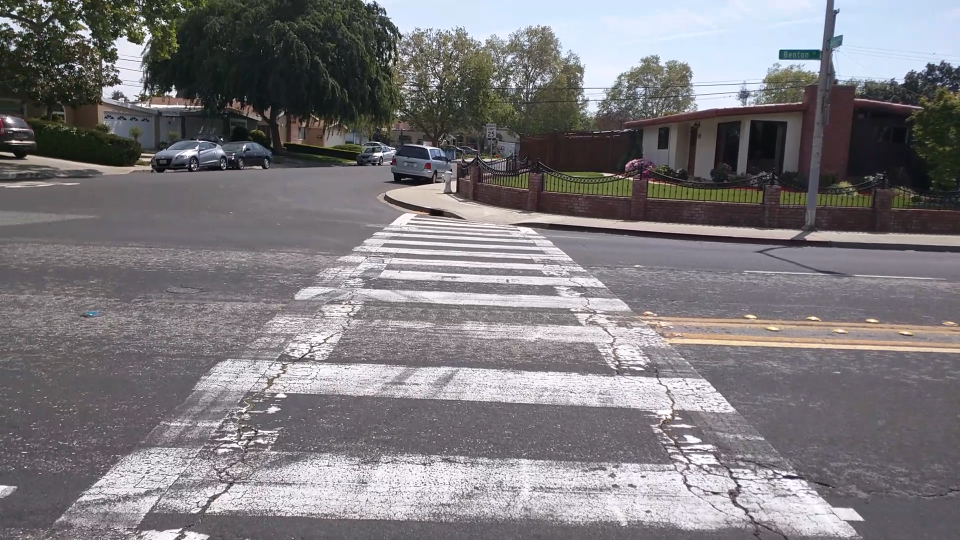
\includegraphics[width=10cm]{PoorlyPaintedHybrid.png}
\captionfonts
\caption[Poorly Painted Hybrid Crosswalk]{Poorly painted hybrid crosswalk}
\label{fig:poorlyPaintedHybrid}
\end{center}
\end{figure}

\clearpage

\begin{table}[t]
    \begin{longtable}{|r|r|r|r|r|r|r|}
    \hline
    Type & \multicolumn{1}{l|}{NN Enabled} & Min & Avg & Median & Max & STD \bigstrut\\
    \hline
    Hybrid & YES & 0.00\% & 58.13\% & 62.50\% & 86.25\% & 30.90\% \bigstrut\\
    \hline
    Hybrid & NO & 15.00\% & 76.46\% & 86.25\% & 98.75\% & 31.18\% \bigstrut\\
    \hline
    Zebra & YES & 55.00\% & 87.64\% & 95.00\% & 98.75\% & 14.82\% \bigstrut\\
    \hline
    Zebra & NO & 62.50\% & 92.22\% & 97.50\% & 100.00\% & 11.85\% \bigstrut\\
    \hline

    \caption{True positive percent results of crosswalk detection categorized by type of crosswalk}
    \label{tab:typeOfCwalk} 
    \end{longtable}
\end{table}

\subsubsection{Effects of Crosswalk Traversal on Accuracy}

As the user walks across the crosswalk, the view of the crosswalk changes and the algorithm needs to continue guiding them. For each crosswalk, 20 frames equidistant throughout the video were used. The expected result of this is that there would be a decrease in true positive rate as the user progresses because there will be fewer stripelets in the image to work with. The data shown in figure \ref{fig:graphOfFrameCount} shows exactly that. The neural network made the rate go down as one would expect, but the drop seemed to increase as the end of the crosswalk was reached. This may be because the training data may be more biased to earlier frames, since the early frames are guaranteed to have more stripelets. In figure \ref{fig:NumStripeletsvsRates}, we can also see that the number of stripelets in each image as the video went on became fewer as the user crossed the crosswalk, but the predictions of the stripelets stayed mostly consistent throughout. 

\begin{figure}[t]
\begin{center}
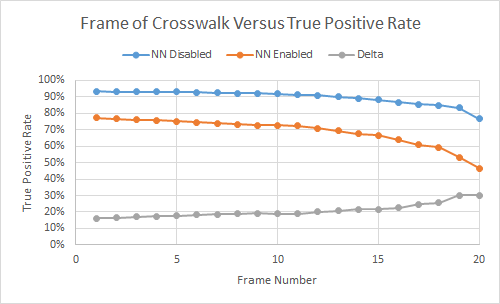
\includegraphics[width=10cm]{FrameResultsGraph.png}
\captionfonts
\caption[Neural Network True Positives Grouped by Frame of Video]{True positive results grouped by frame of video (frame 1 to frame 20)}
\label{fig:graphOfFrameCount}
\end{center}
\end{figure}

\begin{figure}[t]
\begin{center}
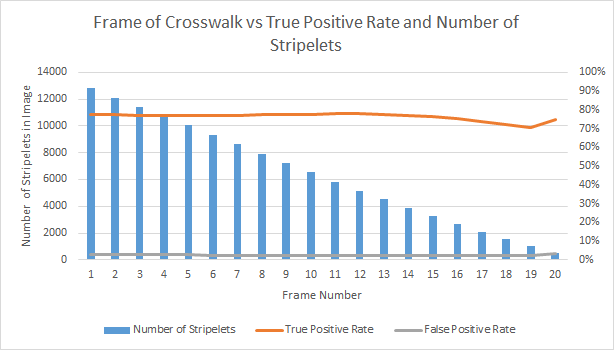
\includegraphics[width=12cm]{NumStripeletsvsRates.png}
\captionfonts
\caption[True and False Positives Grouped by Frame of Video and Number of Stripelets]{True and false positive results grouped by frame of video and showing number of detected stripelets (frame 1 to frame 20)}
\label{fig:NumStripeletsvsRates}
\end{center}
\end{figure}

\clearpage

\subsubsection{Per Crosswalk Analysis of Results}

For this section, the crosswalk videos were grouped by their respective crosswalks, and the non-crosswalk videos were kept as separate groups. The results of this are shown in the appendix tables \ref{tab:appendixcrosswalkresults} and \ref{tab:appendixcrosswalkresultswithoutNeural}, and the summary results are shown in table \ref{tab:crosswalkResultsSummary}. Crosswalks have both true and false positive rates depending on whether they were predicted as being a crosswalk by correct reasoning or not. Videos not containing a crosswalk only have false positives because they cannot contain a crosswalk.  There were a couple outliers in each category (crosswalk vs not) that are included in the dataset, and will be investigated in a later section.

Overall, the average true positive rate of the crosswalk videos was 75.83\% $\pm$ 14.87\% with a standard deviation of 26.28\%. The average false positive rate of crosswalk images was 0.58\% $pm$ .75\% with a standard deviation of 1.33\%. The average false positive rate of the non-crosswalk videos was 1.65\% $\pm$ 1.56\% with a standard deviation of 3.29\%.
The true positive predictions of crosswalks had a rather high standard deviation, which was heavily affected by the one outlier crosswalk, and the false positives were more tightly grouped with a lower standard deviation.

\begin{table}[t]
    \begin{longtable}{|r|r|r|r|r|r|r|}
    \hline
       & Cwalk & Minimum & Average & Median & Maximum & STD \bigstrut\\
    \hline
    True Pos Rates & YES & 0.00\% & 75.83\% & 81.25\% & 98.75\% & 26.28\% \bigstrut\\
    \hline
    False Pos Rates & YES & 0.00\% & 0.58\% & 0.00\% & 5.00\% & 1.33\% \bigstrut\\
    \hline
    False Pos Rates & NO & 0.00\% & 1.65\% & 0.00\% & 12.00\% & 3.29\% \bigstrut\\
    \hline

    \caption[Results summary by video/crosswalk]{Results summary by video/crosswalk. Crosswalks have true and false positives, while non-crosswalk videos only have false positives}
    \label{tab:crosswalkResultsSummary} 
    \end{longtable}
\end{table}



\subsubsection{Yellow Crosswalks}

In order to determine how well yellow crosswalks worked with white crosswalk training data, two yellow crosswalks were tested, one being a standard zebra and the other a hybrid. The hybrid scored 26\% true positive rate, and the zebra scored 66\%, both out of 80 frames. Those results are promising enough to conclude that yellow crosswalks will likely work well with this approach, and would probably improve with yellow crosswalks being included in the training data, due to the differing intensity values between the two colors affecting neural network parameters. 

\subsubsection{Challenging Images and Analysis}

The video with the highest amount of false positives (12\%) was 'NonC Output Night 13,' which was a street being crossed not at an intersection, and with bike lanes going across both sides. The bike lanes and sidewalk were incorrectly matched together, which ended up passing the neural network and the validation as a crosswalk. A couple examples are shown in figure \ref{fig:worstFalsePosPic}, one can see the identified stripelets. More neural network parameters may be able to help remove these from the stripelet set, perhaps something relating to the vertical pixel intensity. 

\begin{figure}[t]
\begin{center}
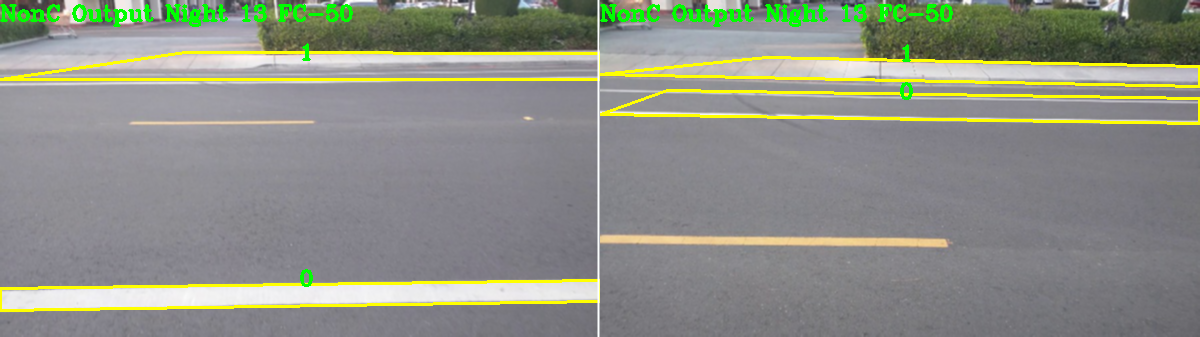
\includegraphics[width=10cm]{NonCWorstCwalk.png}
\captionfonts
\caption[Worst False Positive Examples]{Example frames from 'NonC Output Night 13,' the video with the highest amount of false positives.}
\label{fig:worstFalsePosPic}
\end{center}
\end{figure}

Another video with a high amount of false positives (7\%) was 'NonC Output Night 11,' which is a of a parking lot with many horizontal lines painted throughout.  A few pictures are shown in figure \ref{fig:2ndworstFalsePosPic}. These examples aren't typically what one would expect to see if they were trying to cross the street, but they are lines that look similar to a zebra crosswalk. They could potentially be filtered out by using some sort of expected width vs Y axis level in the image. 

\begin{figure}[t]
\begin{center}
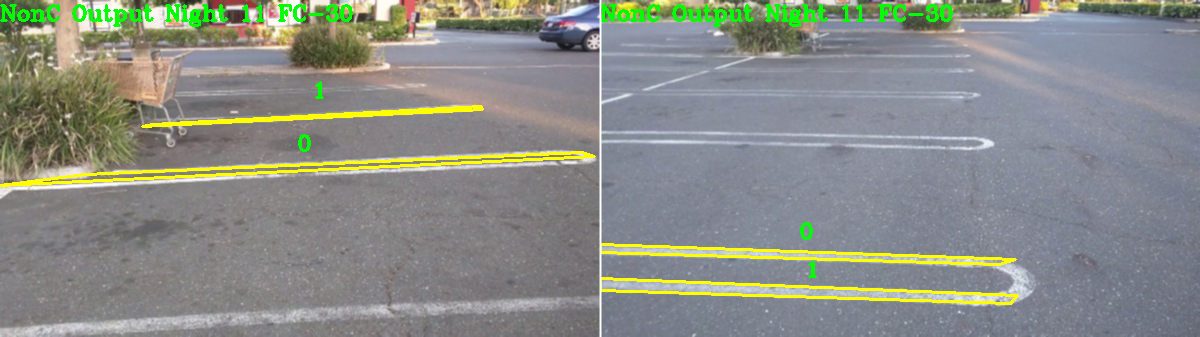
\includegraphics[width=14cm]{NonC2ndWorstCwalk.png}
\captionfonts
\caption[Second Worst False Positive Examples]{Example frames from 'NonC Output Night 11,' the video with the second highest amount of false positives.}
\label{fig:2ndworstFalsePosPic}
\end{center}
\end{figure}

One crosswalk specifically had the worst results by far, 'Night hybrid 3,' shown in figure \ref{fig:worstcwalk}. None of the eighty frames were correctly identified in this crosswalk, whereas the next lowest crosswalk had 57\% of frames correctly identified. The neural network failed to correctly identify enough stripelets in the majority of the images to pass the crosswalk validation. This crosswalk had very odd pavement coloring, which may have contributed to why it failed the neural network.  Potentially this issue could be solved by more training data and including more odd crosswalks such as this one. 

\begin{figure}[t]
\begin{center}
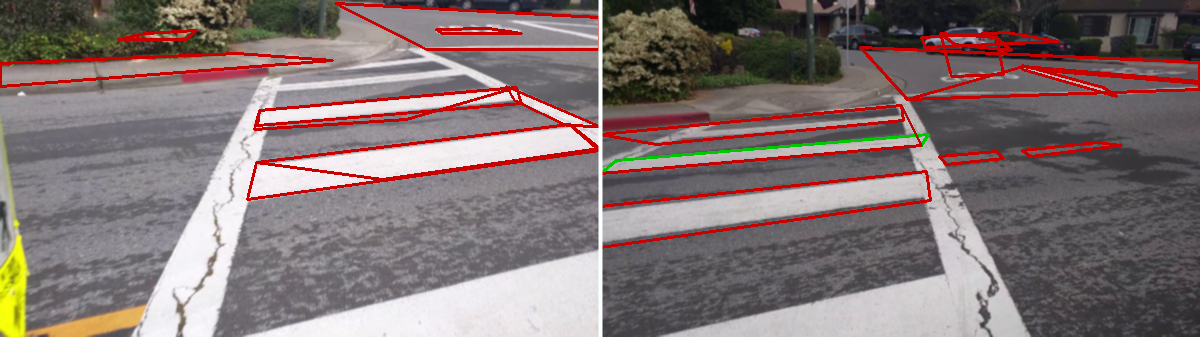
\includegraphics[width=14cm]{WorstCwalk.png}
\captionfonts
\caption[Examples of worst crosswalk]{Example frames from 'Night hybrid 3,' the crosswalk with the worst true positive rate.}
\label{fig:worstcwalk}
\end{center}
\end{figure}

\clearpage

\subsubsection{Overall Results}
%\todo[inline]{JASON - Add another evaluation metric here}  
Over all of the videos, including 1200 crosswalk frames and 970 non-crosswalk frames, and using the neural network to cull stripelets before detection, a q-value of .023 is obtained. When not using the neural network to cull the stripelets, the q-value is .200 (see table \ref{tab:overallresults}). Using the neural network garners an improvement of 985\%. In simpler terms, using neural networks, out of 1000 positively predicted images, only 23 would be false positives versus 200 without using the neural predictions. Figure \ref{fig:CrosswalkTruePosWithAndWithout} shows that for every video, the neural network does drop the positive identifications, but figure \ref{fig:VideoFalsePosWithAndWithout} shows that false positive rates dropped drastically as well for every single case. 


\begin{table}[t]
    \begin{longtable}{|r|r|r|r|}
    \hline
    \multicolumn{1}{|c|}{Neural Network Enabled} & True Positive Rate & False Positive Rate & q-value \bigstrut\\
    \hline
    NO & 91.00\% & 24.88\% & .200 \bigstrut\\
    \hline
    YES & 76.28\% & 2.15\% & .023 \bigstrut\\
    \hline


    \caption[Overall Results of Crosswalk Detection With and Without Neural Networks]{Overall results of crosswalk detection with/without neural networks. Improvement of 887\% in q-value}
    \label{tab:overallresults} 
    \end{longtable}
\end{table}

\begin{figure}[t]
\begin{center}
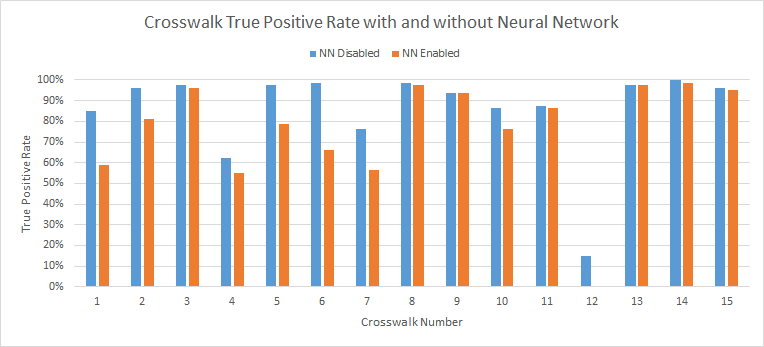
\includegraphics[width=14cm]{CrosswalkTruePosWithAndWithout.png}
\captionfonts
\caption[Crosswalk True Positive Rate with and without Neural Network]{Shows the true positive rates per crosswalk with and without the neural network enabled}
\label{fig:CrosswalkTruePosWithAndWithout}
\end{center}
\end{figure}

\begin{figure}[t]
\begin{center}
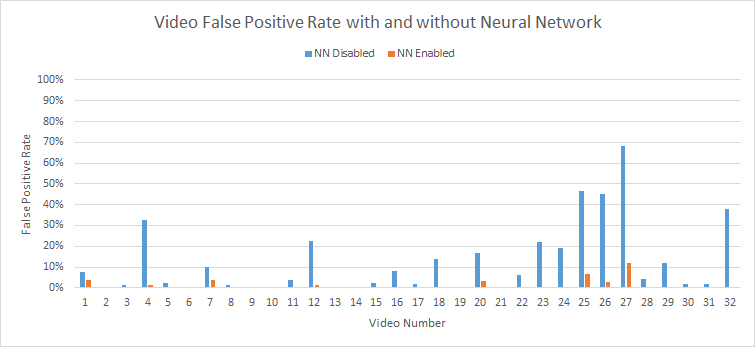
\includegraphics[width=14cm]{VideoFalsePosWithAndWithout.png}
\captionfonts
\caption[Video False Positive Rate with and without Neural Network]{Shows the false positive rates per video with and without the neural network enabled}
\label{fig:VideoFalsePosWithAndWithout}
\end{center}
\end{figure}

\subsection{Crosswalk Boundary Line Drawing Results}

A subset of 180 images were selected to test the crosswalk boundary drawing and had their boundary lines manually drawn. A metric was needed in order to compare the correct line with the estimated line. The metric used involved taking multiple points that were equidistant along the estimated line and finding the normal distance to the manually drawn line. These distances were then summed up to give a general gauge of how close lines were together. Exactly identical lines would have a difference value of zero, while more distinct lines would have greater values. Some example images with their evaluation result values are shown in figure \ref{fig:LinesUsingJustGoodStartAndEnds2}. Overall, the results were rather promising, with the vast majority of lines from images with a recognized crosswalk being close to correct with a median measure of 66 and only 10\% of the lines being over the threshold of 400. As shown in figure \ref{fig:400Metric}, 400 was a generous measure, because even at 400, the lines are still close enough.  If the stripelets are predicted properly, and a crosswalk is recognized, the edges of the stripelets are almost guaranteed to be good metrics of the crosswalk edges.

\begin{figure}[t]
\begin{center}
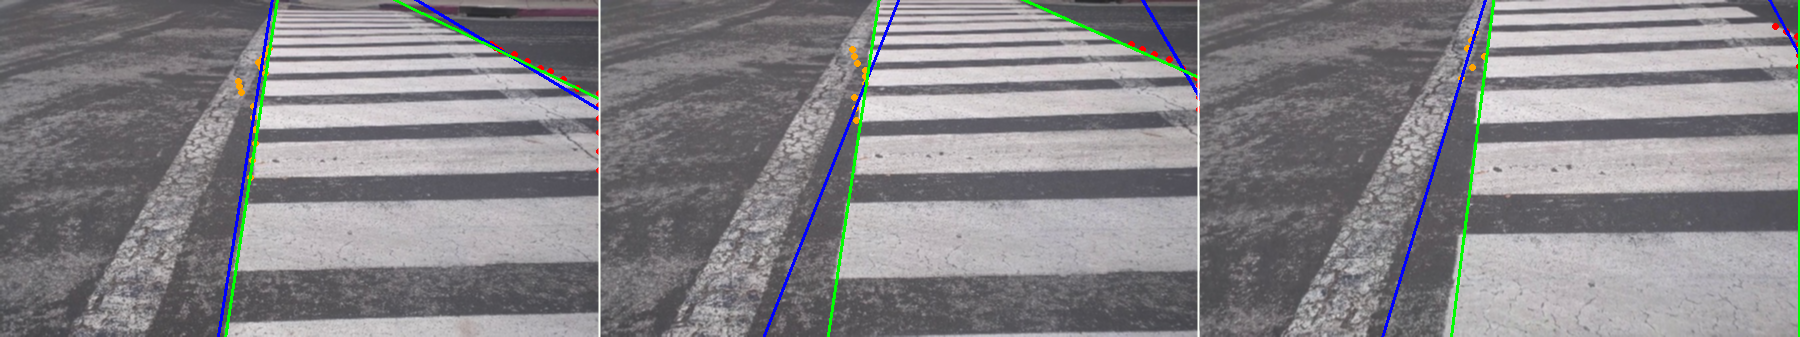
\includegraphics[width=15cm]{LinesUsingJustGoodStartAndEnds2.png}
\captionfonts
%Jeneeplz what term for "left evaluation value"
\caption[Boundary Line Estimation Results]{Orange and red dots are the right and left points used. Green is the manually drawn boundary. Blue is the estimated boundary. Left to right: (a) Left evaluation metric of 38, right 34. (b) left: 178, right: 135. (c) left: 235, right: 90}
\label{fig:LinesUsingJustGoodStartAndEnds2}
\end{center}
\end{figure}

\begin{figure}[t]
\begin{center}
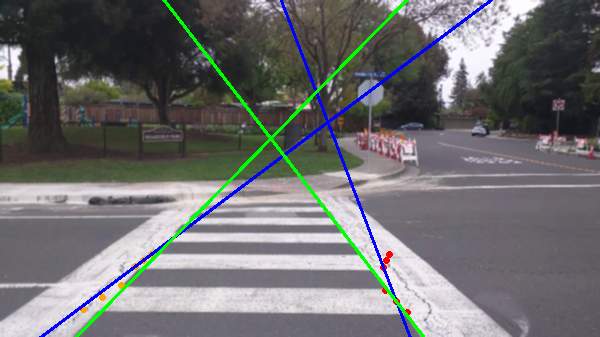
\includegraphics[width=12cm]{400RightSide.png}
\captionfonts
%Jeneeplz what term for "left evaluation value"
\caption[Upper Limit of Boundary Line Metric]{Orange and red dots are the right and left points used. Green is the manually drawn boundary. Blue is the estimated boundary. The evaluation metric on the right side is 400, which is considered the high range of acceptable}
\label{fig:400Metric}
\end{center}
\end{figure}


\chapter{Future Work}
\label{future work}

\section{Conversion to phone app}

The project was written entirely in the C++ libraries provided by OpenCV, which can be ported easily to a mobile app without many changes. Once the algorithm has access to phone sensors, there are opportunities to implement improvements. The current algorithm assumes that the photos are taken parallel to the horizon, but with access to a phone's sensors, the image frames could be adjusted so that they are guaranteed to be in the correct horizontal orientation. The accelerometer and gyroscope sensors could also be used to help track movement as the user crosses a crosswalk. Using sensors, anything above the horizon line could be discarded \cite{Crosswatch2Lane}. Other mobile technologies such as Project Tango's 3-D mapping hardware \cite{projectTango} could be used as well to assist with spatial awareness and other factors such as detecting obstructions that must be avoided. Once the program is converted to a mobile app, there are many interesting ways that it could progress.

\section{Improving Stripelet Detection}

The stripelets that are detected and fed into the neural network could have been more accurate. Different pixel grouping methods to group the detected edges into lines might result in improved stripelets, which would lead to a more accurate input for the neural network and improve detection.

\section{Crosswalks With Shadows}

As this project did not cover crosswalks with shadows, future work could be done to adapt the algorithm so it can work properly with crosswalks that have shadows inside of them. The current algorithm has difficulties with shadows; one issue is that the Hough line transform might have issues because shadows form strong lines, and another being that some of the neural network training parameters might be drastically different with shadows inside of the stripelets. 

One option might be shadow removal algorithms that would remove the shadows so that the main algorithm doesn't have to account for them at all. This could be a good solution because it would require modifying the current algorithm, but might not the fastest. Shadow removal algorithms are quite common, so there would be many different options \cite{shadowRemoval}. Another potential solution would be to modify the current algorithm to handle the shadows. This method would likely involve modifying the Hough lines grouping, as well as using different or modified training parameters for the neural network, and require additional training data including crosswalks with different types of shadows at various times of day. 

\section{More Training Parameters for Neural Network}

The portion of the algorithm that uses neural networks to predict whether or not stripelets are part of the crosswalk would benefit from more investigation into new metrics that would aid the neural network. Investigating new parameters is not a costly procedure in terms of time, and it is not difficult to discover whether a training parameter is working well or not after a single attempt, so it would be worth the investment.  

\section{Improving Detection of Crosswalk Boundary Lines}

Ideally, the algorithm could be improved in detection of the edges of the crosswalk in order to assist the user in navigating across the intersection. One large improvement would be to trend the lines and values along multiple sequential frames to give a more accurate measurement. More experimentation could lead to better methods of doing this as well. 

\section{Use Neural Network for Comparing Two Stripelets in Crosswalk Detection}

Currently, the algorithm is using a few different metrics in order to predict whether two stripelets could be a part of the same crosswalk or not. A neural network could be applied to this decision instead, in order to potentially garner a better result. The same parameters that are being manually used currently would be a good starting point for neural network parameters, as well as the other parameters currently being used by the neural network for stripelet prediction. 

\section{Performance Improvements}

The algorithm contains some areas where the performance could be improved. In this proof of concept, speed isn't as important, so the algorithm is not as optimized as it could be. If it is ported to a phone app, the optimizations would become necessary for a real world usage scenario.

\subsection{Multithreading}
One specific improvement would be to take advantage of multiple CPU cores in order to process multiple frames at the same time. This would improve the throughput and allow greater accuracy due being able to quickly to average the results of frames that are immediately next to each other.
The current implementation running on a decent PC can run at around 1.6 frames per second, and would scale linearly with the number of cores, so if one core is currently 1.6 frames per second, then two cores would be 3.2 frames per second, thus multithreading would give a large performance boost for this application. Multithreading would also be extremely beneficial for the crosswalk side edge detection, because running multiple sequential frames at the same time would allow a more accurate prediction.

\subsection{Finding the Smallest Image Size Necessary}
Another improvement would be to try to find the smallest image size necessary for the algorithm to detect the position of the crosswalk. The smaller the image is, the faster the processing time will be because there are fewer pixels for every operation. This could be discovered by running the algorithm on smaller and smaller crosswalks and finding out when the predictions start degrading to an unacceptable level. The performance would drastically improve, because as the image dimensions are cut in half, the number of pixels are divided by four, which scales almost directly with the runtime because many operations are performed on each pixel, and those operation's runtimes would divided by four. 

\chapter{Conclusion}
\label{conclusion}
%What I did ( couple sentences), why I did it (more), why I think they worked or didn't work  (biggest)
%more about future uses and less about results

This project incorporated neural networks into a process of recognizing zebra stripe crosswalks in images. This process may be effective in aiding a visually impaired user across a crosswalk. 

Neural networks are used in many image processing platforms, but they haven't yet been applied to recognizing zebra crosswalks in this way.

%An improvement of about 887\% increase in q-value was seen when comparing the same code using neural networks vs not using neural networks on the same dataset. With neural networks, there was an increase in runtime due to the calculations required for the neural network, but with optimizations that could be reduced. The dataset used was reasonably large and diverse and garnered decent results. It would definitely be worth looking into this method further for real world use. 

Using the same dataset, a substantial improvement in false discovery rate (887\%) was seen when comparing the same code using neural networks versus without them. There was an increase in runtime due to the calculations required for the neural network inputs, but optimizations could reduce that impact. The dataset used was large and diverse. The results presented in this paper show that using neural networks is a promising tool in zebra crosswalk detection, and is well worth further investigation.







% ------------- End main chapters ----------------------

\clearpage
\bibliography{bibliography}
\bibliographystyle{plain}
%\addcontentsline{toc}{chapter}{Bibliography}

\chapter{Appendix}

    \begin{longtable}{| r | r | r | r |}
    \hline
    Neurons in Hidden Layer & True Positive Rate & False Positive Rate & q-value \bigstrut\\
    \hline
    2  & 72.19\% & 4.33\% & 0.151 \bigstrut\\
    \hline
    3  & 73.35\% & 4.57\% & 0.156 \bigstrut\\
    \hline
    4  & 73.37\% & 4.22\% & 0.145 \bigstrut\\
    \hline
    5  & 73.56\% & 3.38\% & 0.120 \bigstrut\\
    \hline
    6  & 73.27\% & 3.07\% & 0.110 \bigstrut\\
    \hline
    7  & 74.44\% & 2.98\% & 0.106 \bigstrut\\
    \hline
    8  & 73.79\% & 3.03\% & 0.108 \bigstrut\\
    \hline
    9  & 74.56\% & 2.88\% & 0.103 \bigstrut\\
    \hline
    10 & 74.35\% & 2.64\% & 0.095 \bigstrut\\
    \hline
    11 & 75.81\% & 2.72\% & 0.096 \bigstrut\\
    \hline
    12 & 74.69\% & 2.69\% & 0.096 \bigstrut\\
    \hline
    13 & 76.08\% & 2.51\% & 0.089 \bigstrut\\
    \hline
    14 & 75.25\% & 2.38\% & 0.085 \bigstrut\\
    \hline
    \textbf{15} & \textbf{74.42\%} & \textbf{2.36\%} & \textbf{0.086} \bigstrut\\
    \hline
    16 & 75.96\% & 2.81\% & 0.098 \bigstrut\\
    \hline
    17 & 75.29\% & 3.09\% & 0.108 \bigstrut\\
    \hline
    18 & 75.67\% & 2.42\% & 0.086 \bigstrut\\
    \hline
    19 & 76.63\% & 3.02\% & 0.104 \bigstrut\\
    \hline
    20 & 76.13\% & 2.62\% & 0.092 \bigstrut\\
    \hline
    21 & 75.90\% & 2.73\% & 0.096 \bigstrut\\
    \hline
    22 & 75.73\% & 2.74\% & 0.097 \bigstrut\\
    \hline

    \hline
    \caption{Crosswalk identification results from neural network training with different hidden layer configurations}
    \label{tab:NN-HiddenLayersResultsAPP} 
    \end{longtable}



    \begin{longtable}{|r|r|r|r|}
    
    \hline
    Name & Frames & True Positive Rate & False Positive Rate \bigstrut\\
    \hline
    Afternoon hybrid 1 & 80 & 58.75\% & 5.00\% \bigstrut\\
    \hline
    Afternoon hybrid 3 & 80 & 81.25\% & 0.00\% \bigstrut\\
    \hline
    Afternoon zebra 1 & 80 & 96.25\% & 0.00\% \bigstrut\\
    \hline
    Afternoon zebra 3 & 80 & 55.00\% & 1.25\% \bigstrut\\
    \hline
    Afternoon zebra 5 & 80 & 78.75\% & 0.00\% \bigstrut\\
    \hline
    Morning hybrid 1 & 80 & 66.25\% & 0.00\% \bigstrut\\
    \hline
    Morning hybrid 3 & 80 & 56.25\% & 0.00\% \bigstrut\\
    \hline
    Morning zebra 1 & 80 & 97.50\% & 1.25\% \bigstrut\\
    \hline
    Morning zebra 3 & 80 & 93.75\% & 0.00\% \bigstrut\\
    \hline
    Morning zebra 5 & 80 & 76.25\% & 0.00\% \bigstrut\\
    \hline
    Night hybrid 1 & 80 & 86.25\% & 0.00\% \bigstrut\\
    \hline
    Night hybrid 3 & 80 & 0.00\% & 1.25\% \bigstrut\\
    \hline
    Night zebra 1 & 80 & 97.50\% & 0.00\% \bigstrut\\
    \hline
    Night zebra 3 & 80 & 98.75\% & 0.00\% \bigstrut\\
    \hline
    Night zebra 5 & 80 & 95.00\% & 0.00\% \bigstrut\\
    \hline
    NonC Output Afternoon 4 & 50 & -  & 0.00\% \bigstrut\\
    \hline
    NonC Output Afternoon 5 & 50 & -  & 0.00\% \bigstrut\\
    \hline
    NonC Output Afternoon 6 & 50 & -  & 0.00\% \bigstrut\\
    \hline
    NonC Output Afternoon 7 FC-30 & 30 & -  & 0.00\% \bigstrut\\
    \hline
    NonC Output Afternoon 8 FC-30 & 30 & -  & 3.33\% \bigstrut\\
    \hline
    NonC Output Afternoon 9 FC-30 & 30 & -  & 0.00\% \bigstrut\\
    \hline
    NonC Output Morning 2 & 50 & -  & 0.00\% \bigstrut\\
    \hline
    NonC Output Morning 3 & 50 & -  & 0.00\% \bigstrut\\
    \hline
    NonC Output Night 10 FC-200 & 200 & -  & 0.00\% \bigstrut\\
    \hline
    NonC Output Night 11 FC-30 & 30 & -  & 6.67\% \bigstrut\\
    \hline
    NonC Output Night 12 FC-100 & 100 & -  & 4.00\% \bigstrut\\
    \hline
    NonC Output Night 13 FC-50 & 50 & -  & 12.00\% \bigstrut\\
    \hline
    NonC Output Night 5 & 50 & -  & 0.00\% \bigstrut\\
    \hline
    NonC Output Night 6 & 50 & -  & 0.00\% \bigstrut\\
    \hline
    NonC Output Night 7 & 50 & -  & 0.00\% \bigstrut\\
    \hline
    NonC Output Night 8 & 50 & -  & 0.00\% \bigstrut\\
    \hline
    NonC Output Night 9 & 50 & -  & 2.00\% \bigstrut\\
    \hline

    \caption{Results for each crosswalk by name with neural network enabled}
    \label{tab:appendixcrosswalkresults} 
    \end{longtable}


    \begin{longtable}{|r|r|r|r|}
    
    \hline
    Name & Frames & True Positive Rate & False Positive Rate \bigstrut\\
    \hline
    Afternoon hybrid 1 & 80 & 85.00\% & 7.50\% \bigstrut\\
    \hline
    Afternoon hybrid 3 & 80 & 96.25\% & 0.00\% \bigstrut\\
    \hline
    Afternoon zebra 1 & 80 & 97.50\% & 1.25\% \bigstrut\\
    \hline
    Afternoon zebra 3 & 80 & 62.50\% & 32.50\% \bigstrut\\
    \hline
    Afternoon zebra 5 & 80 & 97.50\% & 2.50\% \bigstrut\\
    \hline
    Morning hybrid 1 & 80 & 98.75\% & 0.00\% \bigstrut\\
    \hline
    Morning hybrid 3 & 80 & 76.25\% & 10.00\% \bigstrut\\
    \hline
    Morning zebra 1 & 80 & 98.75\% & 1.25\% \bigstrut\\
    \hline
    Morning zebra 3 & 80 & 93.75\% & 0.00\% \bigstrut\\
    \hline
    Morning zebra 5 & 80 & 86.25\% & 0.00\% \bigstrut\\
    \hline
    Night hybrid 1 & 80 & 87.50\% & 3.75\% \bigstrut\\
    \hline
    Night hybrid 3 & 80 & 15.00\% & 22.50\% \bigstrut\\
    \hline
    Night zebra 1 & 80 & 97.50\% & 0.00\% \bigstrut\\
    \hline
    Night zebra 3 & 80 & 100.00\% & 0.00\% \bigstrut\\
    \hline
    Night zebra 5 & 80 & 96.25\% & 2.50\% \bigstrut\\
    \hline
    NonC Output Afternoon 4 & 50 & -  & 8.00\% \bigstrut\\
    \hline
    NonC Output Afternoon 5 & 50 & -  & 2.00\% \bigstrut\\
    \hline
    NonC Output Afternoon 6 & 50 & -  & 14.00\% \bigstrut\\
    \hline
    NonC Output Afternoon 7 FC-30 & 30 & -  & 0.00\% \bigstrut\\
    \hline
    NonC Output Afternoon 8 FC-30 & 30 & -  & 16.67\% \bigstrut\\
    \hline
    NonC Output Afternoon 9 FC-30 & 30 & -  & 0.00\% \bigstrut\\
    \hline
    NonC Output Morning 2 & 50 & -  & 6.00\% \bigstrut\\
    \hline
    NonC Output Morning 3 & 50 & -  & 22.00\% \bigstrut\\
    \hline
    NonC Output Night 10 FC-200 & 200 & -  & 19.00\% \bigstrut\\
    \hline
    NonC Output Night 11 FC-30 & 30 & -  & 46.67\% \bigstrut\\
    \hline
    NonC Output Night 12 FC-100 & 100 & -  & 45.00\% \bigstrut\\
    \hline
    NonC Output Night 13 FC-50 & 50 & -  & 68.00\% \bigstrut\\
    \hline
    NonC Output Night 5 & 50 & -  & 4.00\% \bigstrut\\
    \hline
    NonC Output Night 6 & 50 & -  & 12.00\% \bigstrut\\
    \hline
    NonC Output Night 7 & 50 & -  & 2.00\% \bigstrut\\
    \hline
    NonC Output Night 8 & 50 & -  & 2.00\% \bigstrut\\
    \hline
    NonC Output Night 9 & 50 & -  & 38.00\% \bigstrut\\
    \hline

    
    \caption{Results for each crosswalk by name with neural network disabled}
    \label{tab:appendixcrosswalkresultswithoutNeural} 
    \end{longtable}





\end{document}